
\documentclass[letterpaper,twocolumn,openany,nodeprecatedcode,breakable,skins,xparse,most]{dndbook}

% Use babel or polyglossia to automatically redefine macros for terms
% Armor Class, Level, etc...
% Default output is in English; captions are located in lib/dndstring-captions.sty.
% If no captions exist for a language, English will be used.
%1. To load a language with babel:
%	\usepackage[<lang>]{babel}
%2. To load a language with polyglossia:
%	\usepackage{polyglossia}
%	\setdefaultlanguage{<lang>}
\usepackage[english]{babel}
%\usepackage[italian]{babel}
% For further options (multilanguage documents, hypenations, language environments...)
% please refer to babel/polyglossia's documentation.

\usepackage{float}
\usepackage[utf8]{inputenc}
\usepackage[singlelinecheck=false]{caption}
\usepackage{lipsum}
\usepackage{listings}
\usepackage{shortvrb}
\usepackage{stfloats}
\usepackage[toc,page]{appendix}
\usepackage{graphicx}
\usepackage{subcaption}


\captionsetup[table]{labelformat=empty,font={sf,sc,bf,},skip=0pt}


% --- Appendix links -------------------------------------------------------
% \appendixlink{label}{Appendix I}{Purgeflame Spells} in the main text, and
% \backlink{label}{Purgeflame} under the appendix heading. Both are banners
% in the book's colours that jump to the other end when clicked.
\usepackage{hyperref}
\hypersetup{hidelinks}
\usepackage{amssymb}
\providecolor{titlered}{HTML}{58180D}
\newsavebox{\apolinkbox}
\newcommand{\apolinkbanner}[3]{% target, small label, title
  \par\addvspace{4pt}\noindent
  \sbox{\apolinkbox}{\begin{tcolorbox}[enhanced, unbreakable, sharp corners, boxrule=0pt,
      frame hidden, colback=titlered!8, left=6pt, right=6pt, top=3pt, bottom=3pt,
      borderline west={2.5pt}{0pt}{titlered}, nobeforeafter, width=\linewidth]
    {\sffamily\scshape\footnotesize\color{titlered}#2\hfill p.~\pageref{#1}}\par
    {\sffamily\bfseries\small #3~\textcolor{titlered}{$\blacktriangleright$}}
  \end{tcolorbox}}%
  \hyperref[#1]{\usebox{\apolinkbox}}\par\addvspace{4pt}}
\newcommand{\appendixlink}[3]{\apolinkbanner{app:#1}{See #2}{#3}}
\newcommand{\backlink}[2]{\apolinkbanner{main:#1}{Back to the main text}{#2}}

\MakeShortVerb{|}

\lstset{%
  basicstyle=\ttfamily,
  language=[LaTeX]{TeX},
  breaklines=true,
}

\title{Apotheosis \\
\large A homebrew campaign}
\author{by "The Charred Eye"}

\begin{document}

\frontmatter

\tableofcontents

\chapter{Changes to the base game}

\DndDropCapLine{T}{}hrough the powers that be, this campaign shall have additional mechanics for the adventurers involved. From Elven princesses of argent starlight to clowns of eldritch fear, this guide to \textbf{Apotheosis} shall outline your unique powers or afflictions.

\section{Homebrew Rules}
This section shall outline universal changes to this campaign's rules from combat, to travel and even roleplay.

\subsection{Travel}
Travel is broken up into three tiers of distance and cost.

\subsubsection{Nearby}
Travel to a place \textbf{Nearby}, will have at least \textbf{1 encounter}, \textbf{1 short rest} \textit{recommended} afterwards, though depending on how fast and what route you take, the encounter can be avoided and the number of resources can increase or decrease. 

\subsubsection{Far}
Travel to a place \textbf{Far} away, will have at least \textbf{2 encounters} and a \textit{required} \textbf{1 short rest} afterwards, though depending on how fast and what route you take, 1 of the 2 encounters can be avoided and the number of resources can increase or decrease.

\subsubsection{Very Far}
Travel to a place \textbf{Ver Far} away, will have at least \textbf{3 encounters}, \textbf{1 long rest} \textit{required} afterwards, though depending on how fast and what route you take, up to 2 encounters can be avoided and the number of resources can increase or decrease.

\subsection{Class Divergence}
Due to the restrictions of roleplay, It shall be allowed for certain classes to use \textbf{variant ability score modifiers} that fit the character better.

\subsubsection{Paladin}

The \textit{spellcasting modifier} for the paladin is \textbf{Wisdom} instead of \textbf{Charisma}.

\begin{DndReadAloud}
   As you will soon discover, this world is ripe with a feast of options and varieties of character flavour heard before only on the lips of a madman!
\end{DndReadAloud}

\begin{figure}
    \centering
    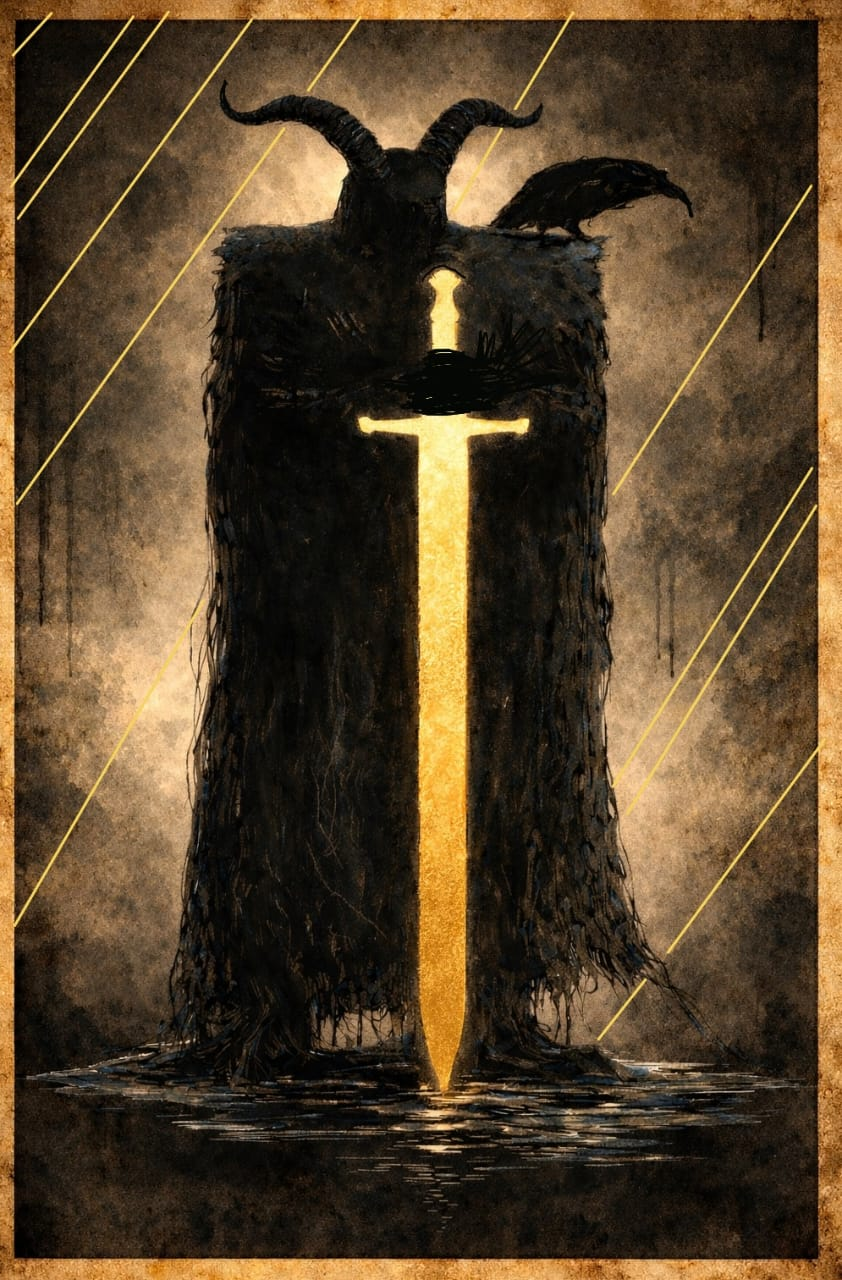
\includegraphics[width=0.7\linewidth]{Images/Black_Knight.jpeg}
    \label{fig:placeholder}
\end{figure}

\begingroup
\DndSetThemeColor[PhbMauve]
\begin{DndSidebar}{Black Knight}
\textit{}
\end{DndSidebar}
\endgroup

\subsubsection{Warlock}

The \textit{spellcasting modifier} for the base warlock is \textbf{Charisma}, though you may upon request choose to use \textbf{Intelligence instead}.

\subsubsection{Sorcerer}
The \textit{spellcasting modifier} for the base sorcerer is \textbf{Charisma}, though if you do not multiclass out of sorcerer, you may request to use \textbf{Constitution} instead.

\subsection{Critcal Rolls}
In the event that \textit{a\textbf{ Natural 20 }}or\textit{ \textbf{Natural 1}} is rolled, the \textbf{\textit{critical success or failure,}} respectively, gets an added effect determined by the \textit{Dungeon Master}.

\subsection{Hybrid Source-Material}
In this campaign, a joint use of the \textit{2014 PHB} and \textit{2024 PHB} shall be used to maximise the roleplaying potential of the adventurers and the world built within this vast tale.

\subsubsection{Species \& Backgrounds}
see the relevant chapter for the custom/adapted \textbf{species} available.

\begin{figure}
    \centering
    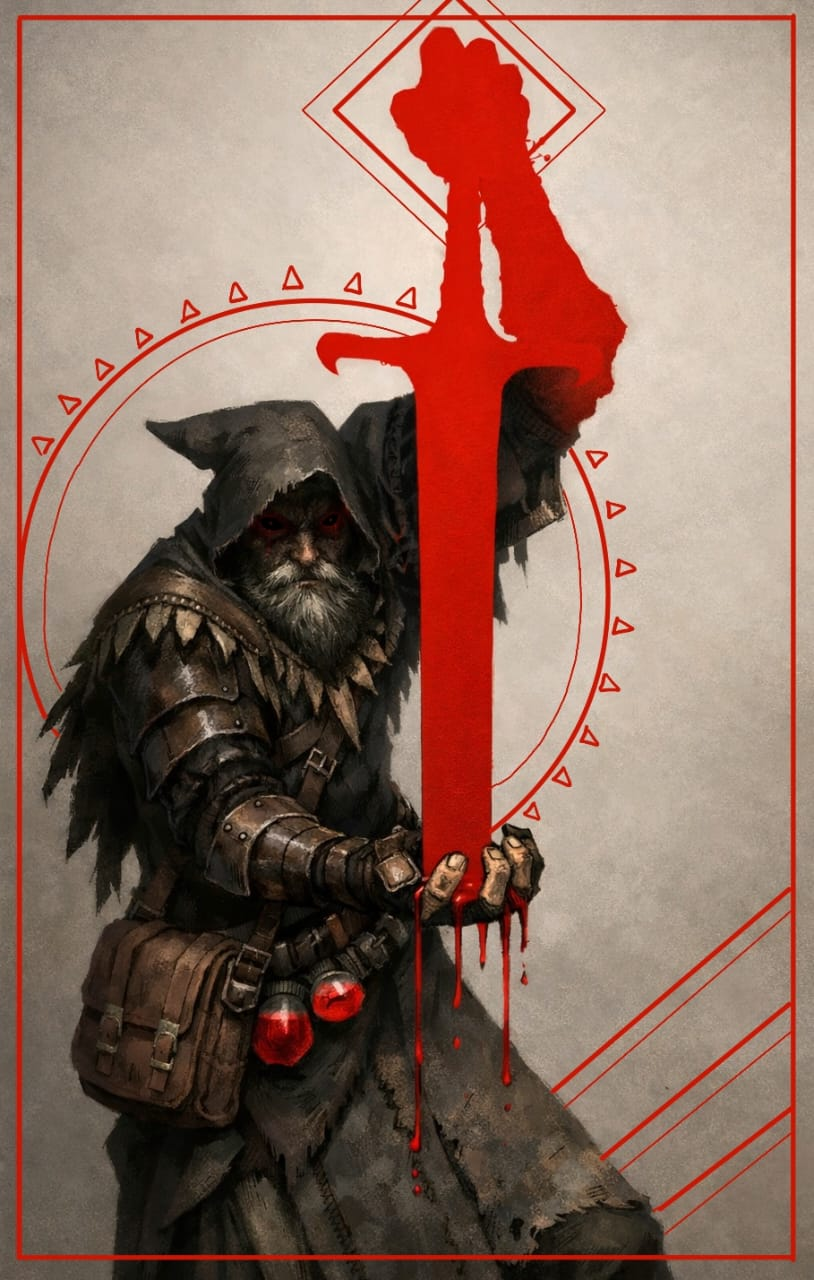
\includegraphics[width=0.75\linewidth]{Images/bloodhunter.jpeg}
    \label{fig:placeholder}
\end{figure}

\begingroup
\DndSetThemeColor[PhbMauve]
\begin{DndSidebar}{Two Halfs of a Whole}
\textit{An organized whole that is perceived as more than the sum of its parts. Wielders of blade \& sorcery...}
\end{DndSidebar}
\endgroup

\subsection{Gestalt Characters}

In this \textit{high-powered campaign variant}, characters essentially \textit{take two classes at every level}, choosing the best aspects of each. The process is similar to multiclassing, except that characters gain the \textbf{full benefits of each class at each level}. if the two classes you choose have aspects that overlap , \textbf{\textit{you choose the better aspect}}.\textbf{\textit{ The gestalt character retains all aspects that don’t overlap.}}

This feature can only be invoked \textbf{at the start of the campaign} and upon the \textbf{Dungeon Master's discretion}. It is required for the party to have \textbf{three or fewer members} generally.

\subsubsection{Hit Dice}
When determining hit die pool and your hit point maximum, you would take whichever hit die would give you the \textbf{most benefit}. For every subsequent level after making your character, look at the two classes you have selected, and \textbf{choose whichever class gives the largest hit die} and add to your hit die pool, and to determine your new Hit Point maximum. Do note that you still only gain \textbf{1 hit die}, and \textbf{1 hit die worth of maximum HP} with a gestalt character.

\subsubsection{Proficiency Bonus}
When determining your proficiency bonus, you still look at your \textbf{current character level} as if you were a non-gestalt character, \textit{as per normal}.

For example a 5th level gestalt character might be a 5th level Fighter and 5th level wizard, but they are still a \textbf{5th level character}.

\subsubsection{Saving Throws}
To determine your\textit{ saving throws}, you do so by taking both starting classes saving throws and \textit{combining those into a list}. You then \textbf{choose two} of those saving throws from that list with which to be proficient in. (IE Fighter/Rogue would \textbf{choose 2 from Str/Dex/Con/Int})

\subsubsection{Class Features}
For Gestalt character, you gain \textbf{all class features \& restrictions} from each of your classes. If your two classes would grant the \textbf{same feature}, such as extra attack, or spell slots, use whichever class which would grant you the \textbf{best bonuses}.

For Example, a Paladin/Sorcerer would determine their spell slots \textbf{as per the Sorcerer spell slot table}. For Example, a Fighter/Barbarian would determine their extra attack from \textbf{Fighter}.

\subsubsection{Spell Casting}

As already stated above, when determining your spell slots you use the class which would give you the \textbf{most spell slots}. The one exception to this is \textbf{Warlocks with any other spell casters}. As warlocks do not gain the "Spell casting" feature and instead get "Pact Magic" a Warlock/Caster would get \textbf{both the spell slots from Warlock and spell slots from the caster}.

When determining which spells you can cast/prepare/know, do so \textit{as written for each class as normal} for your given level. This means that if you have \textbf{two different casters} you would prepare spells for \textbf{both classes as normal}. This in turn grants you a \textit{much wider spell list} from which to choose from over the course of your \textit{"adventuring day"}, but does not grant you \textbf{extra spell slots} (with the above stated exception of warlocks and pact magic).

\subsubsection{Ability Score Improvement}
Ability Score Improvement (ASI for short), has a \textbf{major change} from the normal ruleset when making a Gestalt Character. The ASI's from levels \textbf{4, 8, 12, 16, 19} are \textbf{half as effective}. Meaning that if you wanted to increase your ability scores you would only gain \textbf{1 ASI point} for each "ASI" you would gain at the above levels. If you are using feats you must expend \textbf{BOTH of your ASI's} in order to select a feat.

The exception to this rule is any ASI gained from the \textbf{non-standard list} (\textbf{4, 8, 12, 16, 19}), such as from Fighters levels \textbf{6/14}, or rogues from level \textbf{10}. These "\textit{non-standard}" ASI levels work \textbf{as normal}, granting you \textbf{2 ASI points}, or the ability to select a feat (if allowed in your game).

\begin{figure}[H]
    \centering
    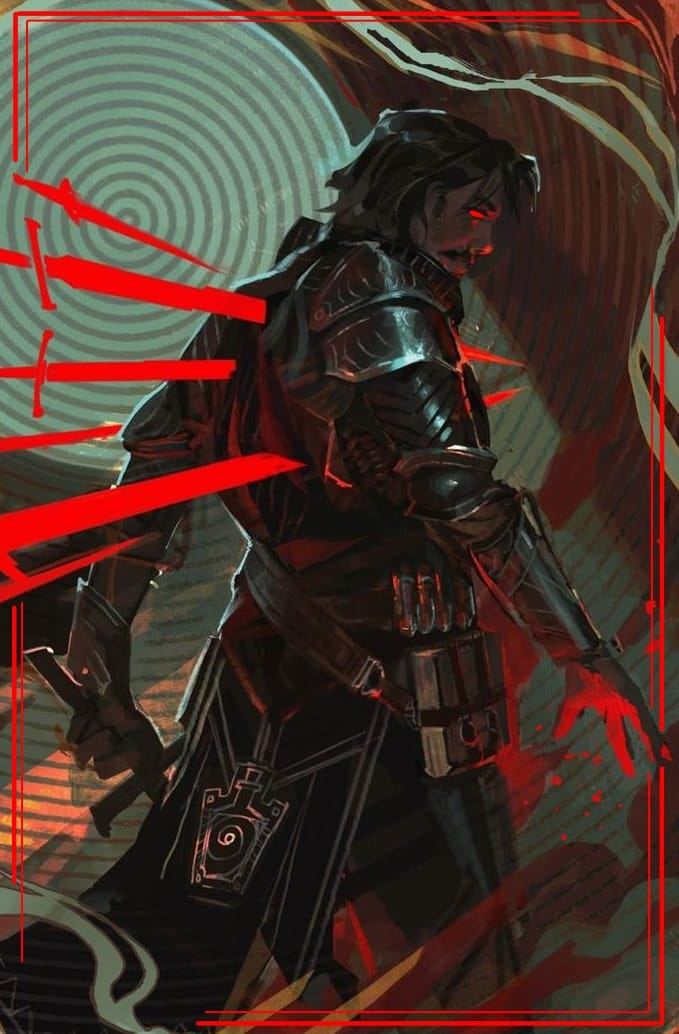
\includegraphics[width=0.7\linewidth]{Images/gestalt.jpeg}
    \label{fig:placeholder}
\end{figure}

\begingroup
\DndSetThemeColor[PhbMauve]
\begin{DndSidebar}{Death is never the end...}
\textit{}
\end{DndSidebar}
\endgroup

\subsection{Heroic Death \& Act of Valour}
These story-driven options to enrich combat do not replace any previous features, yet serve as narrative engines to offer variety to downed party members or avoid TPKs.

\subsubsection{Act of Valour}
Once per campaign, in the place of getting downed at 0 hit points, you can instead opt to\textit{ stand and fight at the cost of all of your inspiration points, regardless of how many you currently have}. 

For three rounds you continue to fight and afterwards you \textit{fall unconscious} and gain the effect:\textit{ Weary}.

You \textit{regain all of your special dice, spell slots and class-specific resources} and any unused features gets depleted again when the effect ends. You can have negative hit points if damage is taken while in this state.

If you are healed by a spell that restores more hit points than your negative hit point value, you do not fall unconscious and continue fighting.

\textbf{Weary:}

Due to fighting past your limits, you are now \textit{dangerously exhausted and have a -4 to all ability checks and attack rolls until your next long rest.}

\subsubsection{Heroic Death}
Once per campaign, irregardless of whether you used the Act of Valour feature, you can choose to keep fighting for 3 rounds after getting downed. You regain all spell slots, class features and special resources as though you were making an Act of Valour.

In addition to this, you add your proficiency bonus to all attack rolls and add it to your spell save DC for the purpose of empowering your spells that require a saving throw. 

You cannot be healed when damage is taken during this state, and you can only be revived with a scroll or spell of true resurrection. 


\subsection{Group Rolls}
When the adventuring party is faced with difficult checks that might not be individually made, the group can add all of their rolls together against a combined DC to utilise everyone's bonus.

\subsubsection{Stealth}
When a party sneaks, instead of individual stealth checks, the whole group rolls and the scores add up to a party sneak score. Failing this ability check, reveals the whole party from stealth. The choice between individual and a group stealth, must be decided and roleplayed beforehand.

\subsubsection{Obstacles}
When the party must overcome obstacles they add all relevant skill check results together against a combined DC to overcome the challenge.

\subsubsection{Bartering}
The whole party barters together using the resultant charisma bonus to skill checks and discounts of the group combined, however the items must be shared and the whole party must unanimously decide to purchase the item.

\begin{DndReadAloud}
    
\end{DndReadAloud}

\chapter{Species \& Backgrounds}

\section{Species}
\DndDropCapLine{T}{}he custom or adapted species section in this grimoire serves to elaborate on the history of the world and its denizens. They are \textbf{Seraphs, Elves, Drakeborn, Orqs, Dwerfens , Golyaths, Halflings, Tieflings,} and of course \textbf{Humans}.

\begin{figure}[H]
    \centering
    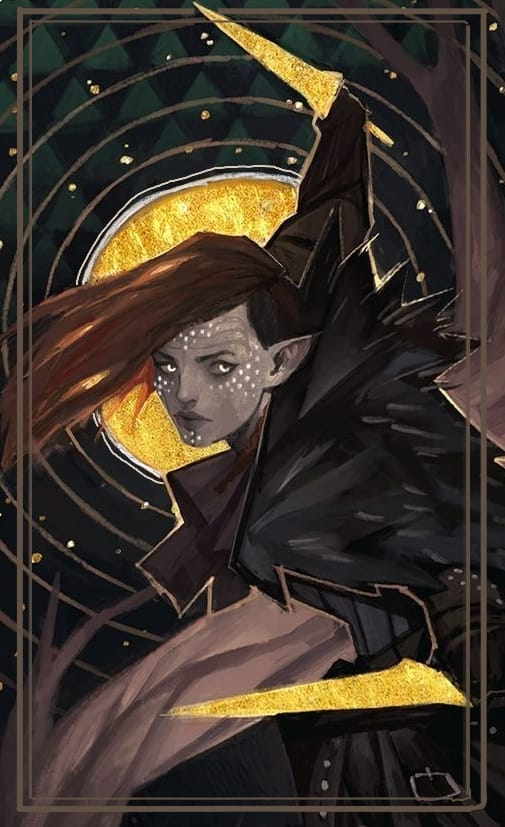
\includegraphics[width=0.58\linewidth]{Images/drow_assassin.jpeg}
    \label{fig:placeholder}
\end{figure}
\begingroup
\DndSetThemeColor[PhbMauve]
\begin{DndSidebar}{The Knives in the dark...}
\textit{}
\end{DndSidebar}
\endgroup

\subsection{Elves}
Descendent from the \textbf{primordial elves} that first inhabited the known world, they are the main humanoids ruling over their respective kingdoms in the far and not so far corners of this campaign. With \textit{ears like blades and varying adaptations to their namesake environs}, elves are the most versatile and abundant race second only to \textbf{humans}.

\subsubsection{High Elf}
\textit{Gladiatorial and Greco-Roman culturalists of decadent design}, \textbf{high elves} rule the \textbf{largest kingdom of Romulon}, the political and religious nexus of the known world. With golden-metallic skin and thick fair hair, some argue they are the most beautiful of the modern elves.

\subsubsection{Dark Elf \textit{(Drow)}}
The deep elves of the\textbf{ underdark} differ from their fair-skinned cousins only in hue, \textit{with brass and bronze skin and pale grey or dirty blonde hair, these elves boast bioluminescent marks that match their red and purple glowing eyes} made to see the \textbf{underdark's} darkest corners. Predominantly from the city \textbf{near the undersea - Latibulus}.

\subsubsection{Wood Elf \textit{(Dryad)}}
These primal Elves of the wooded variety embody nature like none other, bound by the \textbf{verdant oath}, these elves may not harm nature by any means. \textit{With horns and pale green, marked skin, these elves have lost their metallic glamour in favour of pragmatic features to hunt}. Their main settlements are sprinkled wherever there are forests and jungles, but the biggest by far is \textbf{Kaer Holte}, better known as the \textbf{"Hollow Keep"} within the \textbf{Phenozimal Jungle}.

\subsubsection{Snow Elf}`
An offshoot of the wood elves, \textbf{snow elves} were an \textit{advanced civilization of astrologers and scholars of the heavens}; \textbf{occult interference rendered the race lost to time}. \textit{With pearlescent hair, metallic silver skin, claws and dark eyes like the night sky, they branched when the wood elves were still nascent to the primal elves}. The lost citadel of \textbf{Tír Astrada} was the home the original royal line, sadly it is a plundered mess of ruins in modern times.

\subsection{Elf Traits}
The base Elven traits and characteristics are the same as in the \textit{2024 PHB}.

The subspecies of Elf you are determines the evolutionary magicks you possess. The spells available to you manifest at levels 1, 3 and 5 as you mature in power.

These are the same as in the \textit{2024 PHB}, for \textbf{snow elves} you learn the \textit{light cantrip} and gain \textit{resistance to frost damage} at level 1, you additionally learn \textit{ice knife} and \textit{mirror image} at levels 3 and 5 respectively. 

The race is \textit{only playable at the discretion of the game master} as they are \textbf{presumed extinct}.

\begin{DndReadAloud}
   The Elves were the original race of beings on this world, it is only with the arrival of the humans in a cosmic event that the other exotic species arose from their enigmatic roots.
\end{DndReadAloud}

\subsection{Dwerfen}
The "Dwarves" or the more technically correct term in the current world is that of the \textbf{Dwerfen}. \textit{Reclusive and Greedy engineers of brass marvels}, these Persian inspired denizens of the \textbf{Deep Roads} live much \textit{farther underground} than the \textbf{Drow} and almost never surface unless for \textit{political or trade reasons}. \textit{Elf-like in appearance, this species bears no ties to the Elves, instead originating from far below the world's crust}.

Generations of proximity to lyrium ore veins have made dwarves naturally resistant, though not completely immune, to its effects. Even their resistance is only skin deep, as direct exposure of raw lyrium to open cuts, inhalation, or contact through the eyes or mouth leaves them vulnerable to side effects. The side effects are usually non-lethal so long as the amount of lyrium and frequency of invasive exposure is minimal. Surface dwarves lose this resistance over time.

\subsection{Orqs}
Wood Elves \textit{cursed to savagery in opposition to their intrinsic harmony with nature}, \textbf{Orqs} resemble their Elven ancestors faintly, having traded their \textit{antler horns for wolven canines and ridged faces} and a hunger for conquest.\textbf{ The Pariah-Folk} are found in \textit{dessicated forests and torn-down jungles}, used to fuel their engines of war.

\subsection{Golyaths}
Towering over most folk, \textbf{golyaths} are distant \textit{de-
scendants
of
giants, a primordial demi-deitic race of beings that with time became the landscape we now find ourselves traversing. Though mostly extinct, some giants can be found in the extrema of the worlds elements}. Each \textbf{golyath} bears the favours
of
the first
giants. Favours that
manifest in various
supernatural boons, including the ability to quickly
grow and temporarily approach the height
of
golyaths' gigantic kin.
\textit{Golyaths have physical characteristics that are
reminiscent
of
the giants in their family lines}. For
example, some \textbf{golyaths} look like stone giants, while
others resemble fire giants.

\subsection{Drakeborn}
The \textbf{Drakeborn} are an \textit{oviparous race of scaled humanoids}. Their \textit{draconic features mirror their culture's archaic medieval dogma}, although curiously \textbf{hive-minded}, the there \textit{is room for individual ambition and emotion}. Whether humans were \textit{cursed or gifted with the essence of dragons} is unknown, as is most of their culture. They are themed for the types of dragons and vary in how lizardlike they appear. \textbf{They use the abilities of the Forgotten Realms' Dragonborn}.

\begin{figure}[H]
    \centering
    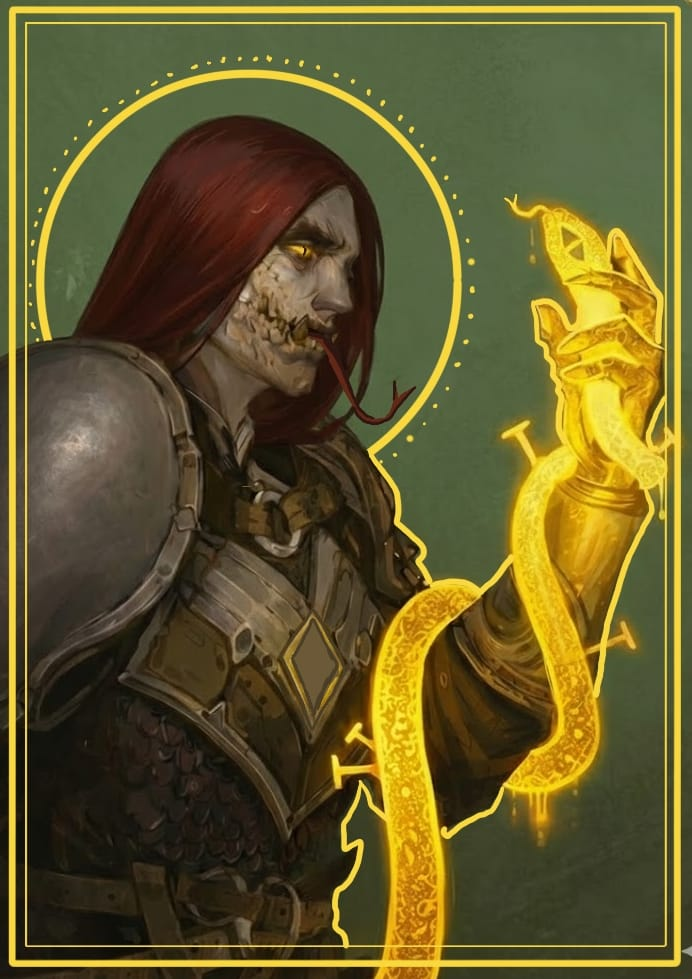
\includegraphics[width=0.64\linewidth]{Images/argonian.jpeg}
    \label{fig:placeholder}
\end{figure}

\begingroup
\DndSetThemeColor[PhbMauve]
\begin{DndSidebar}{Scaled and Cold-blooded}
\textit{Hivemind-driven Scaled Ones, known as the Drakeborn.}
\end{DndSidebar}
\endgroup

\subsection{Halflings}
Small critters from the \textbf{Everglade}, \textit{a permanently spring/autumnal meadowland perfect for farming and respite.} Generally kind and unambitious.

Anyone
who has spent
time around \textbf{halflings}, particularly halfling
adventurers
, has likely witnessed
the \textit{storied "luck
of
the halflings"} in action. When a
halfling is in
mortal danger
, \textit{an unseen force seems
to intervene on the halfling's behalf}.

\subsection{Humans}
\textbf{Humans }are as
\textit{varied as they are numerous}, and they endeavor to
achieve as much as they can in the years they are
given.\textit{ Their ambition and resourcefulness are commended, respected, and feared by all races, though the individual human is more a blank canvas than a creature of great power.}

\subsection{Seraphs}
\textbf{Seraphs} \textit{are mortals
who carry a greater spark of the outer deities within their
souls}. Whether descended from an angelic being or
infused with celestial power, they can \textit{arc that essence outward
to bring light, healing, and heavenly fury. Additionally they exhibit supernatural traits such as resistances and enhanced senses}.
However you are inclined to believe, these divine traits often \textit{manifest in biblically frightening ways} as supposed to the usual winged elven appearance.

\begin{figure}[H]
    \centering
    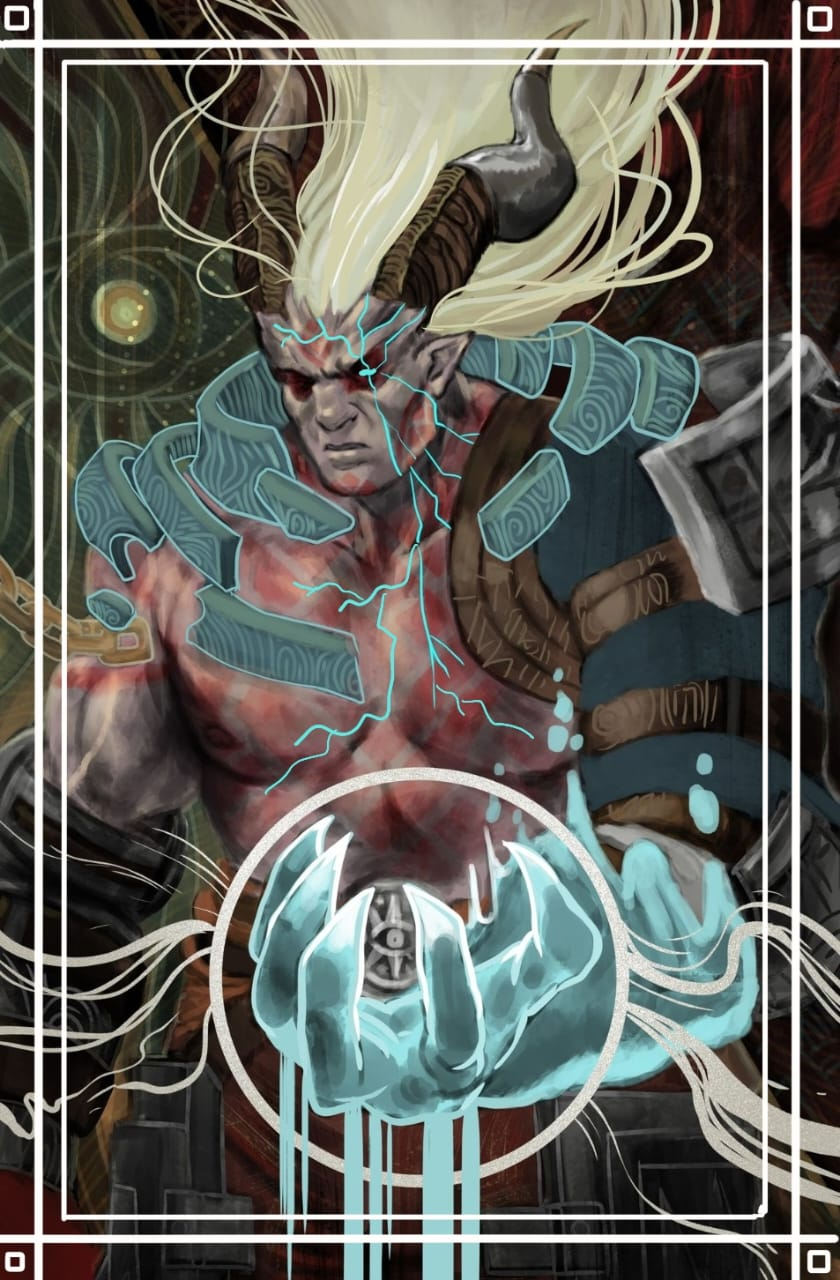
\includegraphics[width=0.64\linewidth]{Images/saarebas.jpeg}
    \label{fig:placeholder}
\end{figure}

\begingroup
\DndSetThemeColor[PhbMauve]
\begin{DndSidebar}{Saarebas or "Dangerous One"}
\textit{The Abyssal Tieflings borne of \textbf{Dremoric influence} have unified under a banner of \textbf{strict religion} in opposition to their evil origin.}
\end{DndSidebar}
\endgroup


\subsection{Tieflings}
Lineages cursed through \textit{occult dealings or less than savoury unions}, \textbf{Tieflings} bear resemblance to christian depictions of demons, though they vary in origin and diverge to appearances alien or common. The source of a lineage determines the appearance and most members of these ethnicities, shunned by the other cultures, have \textit{gathered into kingdoms and formed unique cultures of their own}.

\subsubsection{Infernal}
\textbf{Infernal Tieflings}, shunned by all god-fearing people, are \textit{Luciferian individuals in appearance alone}, for they are \textbf{not intrinsically evil at all}, merely an unfortunate byprodcut of their circumstance. Some adhere to the stereotype, whether it be nature or nurture, and reinforce the stigma binded to them. \textit{Horns, spines, tails, golden eyes and a faint odour of sulphur are common physical features} to these creatures that trace their ancestry to \textbf{Devils} of the \textbf{Nine-Hells}. These tieflings classify as \textbf{\textit{fiends}}.


\subsubsection{Abyssal}
The beastly, muscular tieflings of \textbf{Dremoric} origin have collected to a \textit{large empire of lawful strictness} know as the \textbf{Vashoth or "Grey Ones"} symbolising their \textit{neutral choice of alignment}, \textit{rejecting the chaotic evil nature of their} \textbf{Dremoric} \textbf{ancestry of }\textbf{Oblivion}. The females appear \textit{more alienlike} and exhibit \textit{extra eyes and an improved perception}. These tieflings classify as\textit{\textbf{ fiends}}.

There are \textbf{no Abyssal Tiefling wizards}\textit{ since magic is outlawed}, however those \textbf{born with magical powers are shackled} and \textit{forced to imbibe}\textbf{ Lyrium}, \textit{a bluish crystal substance that empowers a spell to no longer require any components and able to be cast with instinct alone}. These abominations are known as \textbf{Saarebas}.

\begin{DndReadAloud}
   The Elves were the original race of beings on this world, it is only with the arrival of the humans in a cosmic event that the other exotic species arose from their enigmatic roots.
\end{DndReadAloud}

\subsubsection{Cthonic}
"Gravely" in appearance and tragically misunderstood, the \textbf{Chthonic tieflings} are the\textit{ most terrifying in appearance, with horns that seemingly grow out the eye-sockets}. They are \textbf{physically blind}, but are able to sense their surroundings magically and have effective \textbf{blindsight to a range of 15 m} around them. Just like their \textbf{infernal and abyssal cousins}, \textit{they contain no malignant nature from birth and are generally the kindest of the tieflings despite their melancholic circumstance}. \textit{Favouring jewelry and fancy clothes to appear less monstrous}, these tieflings often own large businesses with less horrific looking races performing trade for public relations. These tieflings classify as \textbf{\textit{aberrations}}.

\begin{figure}[H]
    \centering
    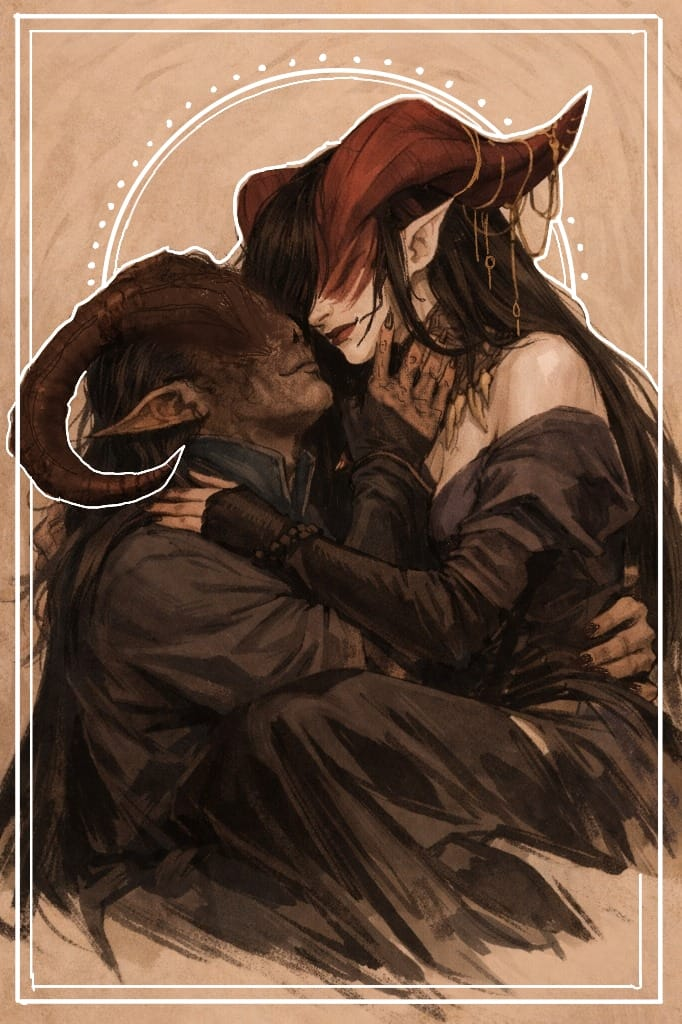
\includegraphics[width=0.64\linewidth]{Images/cthonic.jpeg}
    \label{fig:placeholder}
\end{figure}

\begingroup
\DndSetThemeColor[PhbMauve]
\begin{DndSidebar}{A face that only a mother could Love}
\textit{The \textbf{Cthonic Tieflings} are the least common and most misunderstood, but to understand another deeply is to see them, to Love.}
\end{DndSidebar}
\endgroup

\section{Half-Blood Species} 
\DndDropCapLine{H}{}\textit{\textbf{alf-bloods}} are the result of a \textit{union between two species} and can be a \textbf{mix of any two besides \textit{seraphs}} to diversify gameplay. The appearance includes features from both the parents chosen by the player and must fit according to the abilities chosen associated with them. How the racial abilities are chosen follow according to set rules and the player character does \textit{not retain every single feature from both parents, but rather a mixture of the two.} If chosen during character creation.

\subsection{Base Features}
Due to your genetic diversity, you gain \textbf{immunity to most common diseases},\textit{ with the exception of magic illnesses} and the a \textit{decreased chance to be affected by race-altering curses such as vampirism, this is played by rolling a \textbf{D20} with disadvantage against a \textbf{DC10}}. If the check is failed, you become severely weakened until long rest and upon a critical failure you receive a \textbf{permanent debuff at the DM's discretion} related to the failed transformation.

\subsection{Inherited Features}
List each parent’s racial traits exactly as written, treating each bullet as a separate trait. Your hybrid gains a number of racial traits equal to the higher of the two parents’ trait counts, chosen from either parent, with the restriction that you must take at least one trait from each parent. All chosen traits are gained exactly as written. You do not gain any traits you did not choose, and you never gain more total traits than the higher-trait parent provides.

\subsection{Size \& Speed}
Your walking speed is the average of your two parent species' walking speeds, rounded down to the nearest 5 feet. For any additional movement speed (climb, swim, fly, burrow), take the same average; if only one parent has that movement type, treat the other as 0, so the result may be reduced or drop to 0 after rounding (and you then don't have it).

Your size is determined by your parents' sizes: if they match, you are that size; if they're one size category apart (Small/Medium or Medium/Large), you are the smaller; if they're two apart (Small/Large), you are Medium.

\begin{DndReadAloud}
   The Elves were the original race of beings on this world, it is only with the arrival of the humans in a cosmic event that the other exotic species arose from their enigmatic roots.
\end{DndReadAloud}

\newpage

\section{Variant Species}
\DndDropCapLine{V}{}\textbf{ariant Species} are supernatural augmentations laid over a character’s base race, meant to represent curses, blessings, bloodline mutations, divine meddling, magical corruption, or other transformative forces that set an individual apart from ordinary folk.

In most cases, a Variant Species does not replace the traits of the base chosen species, but instead adds new features, modifies existing capabilities, or imposes thematic drawbacks that reflect the nature of the transformation.

\subsection{Dhampir}
Poised between the worlds of the living and the dead, \textbf{dhampirs} retain their grip on life yet are endlessly tested by vicious hungers. Their ties to the undead grant dhampirs a taste of a vampire’s deathless prowess in the form of increased speed (extra 10 m), darkvision, and a life-draining bite. Generally Born of a vampiric woman and a human or dhampir father, these deathless trace their lineage back to the original unnamed Vampire twins; brothers who saught out immortality without the severance of their souls. However rare, dhampir can be created when a human drinks the blood of a vampire and survives. The bite attack starts out with a base damage of \textbf{2d4} that increases to \textbf{2d6, 2d8} and \textbf{2d10} at \textit{levels 4, 8, and 12 respectrively}, that heals the player for the damage dealt.

\subsubsection{Crystalline}
Iridescent and brittle-skinned and incomprehensably beautiful, these dhampir are more durable than their bat-like cousins and generally blend into society better, though crystalline dhampir do not wither beneath the day but instead gleam all the brighter in it, their skin casting prismatic light like living crystal and marking them at once as something not wholly mortal. They gain the \textbf{feat: }\textbf{tough}, but become \textbf{vulnerable to Thunder Damage}.

\subsubsection{Chiropterine}
Bat-like and hairy, though still human-esque in appearance, these dhampir are more animalistic and gain heightened awareness and keen reflexes; marked by its more bestial caste: furred limbs, membranous ears, sharp features, and the restless, twitching alertness of a hunting thing.. They gain the \textbf{dread ambusher feature from Gloomstalker Rangers} but become \textbf{vulnerable to radiant damage}.

\begin{figure}[H]
\centering
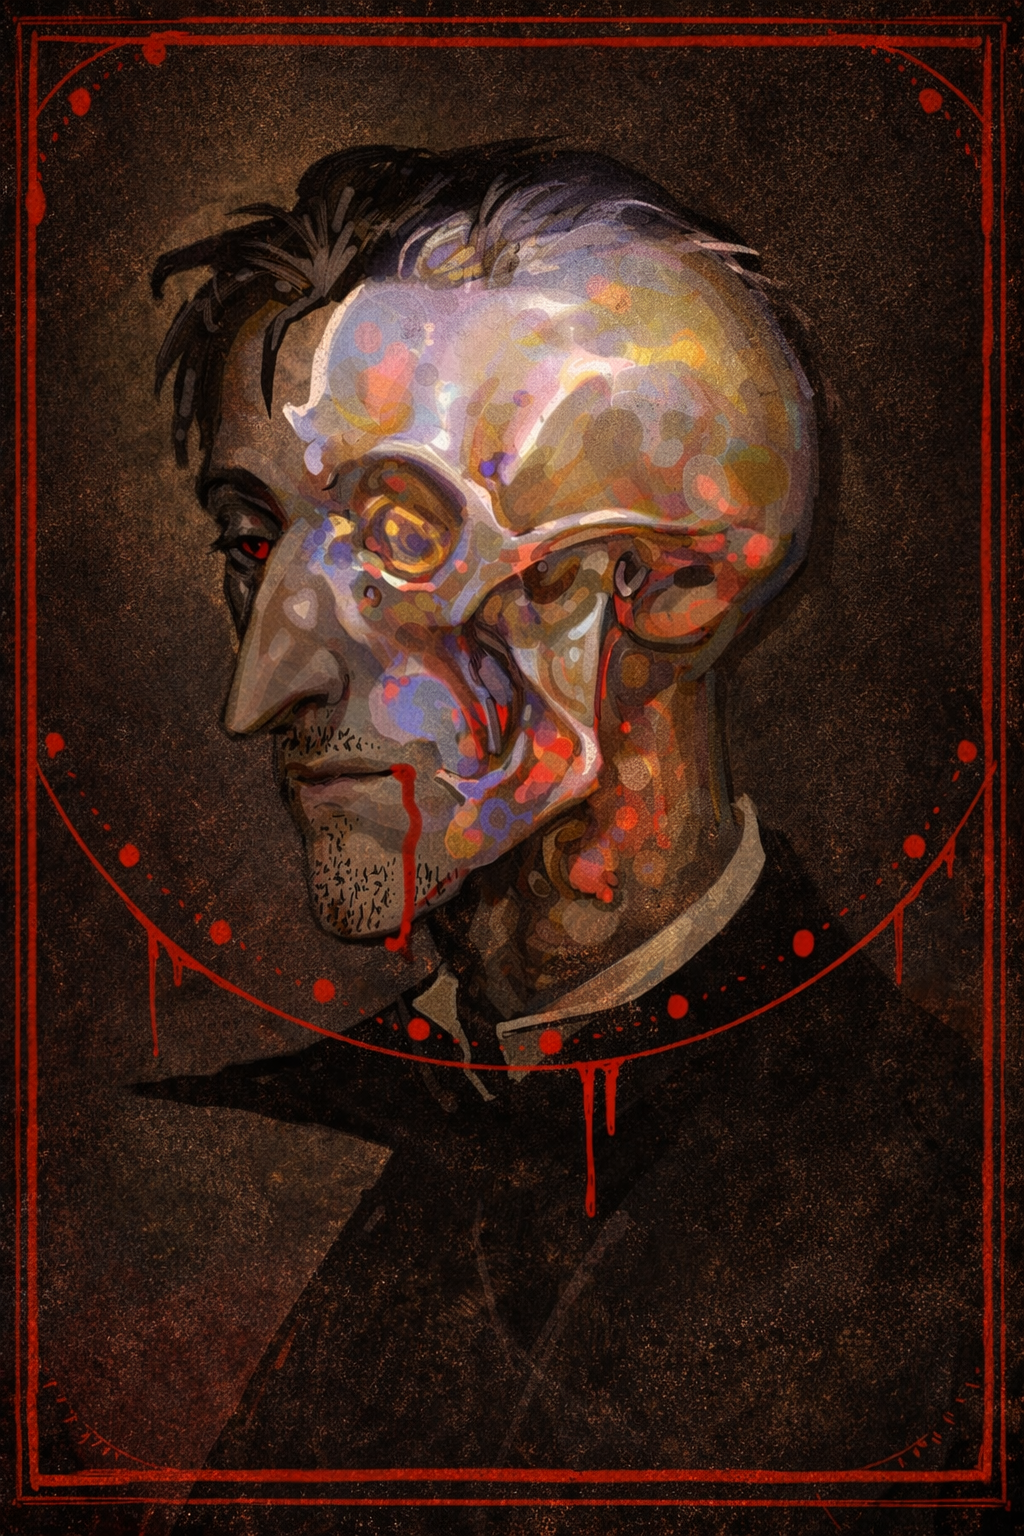
\includegraphics[width=0.225\textwidth]{Images/Dhampir.png}
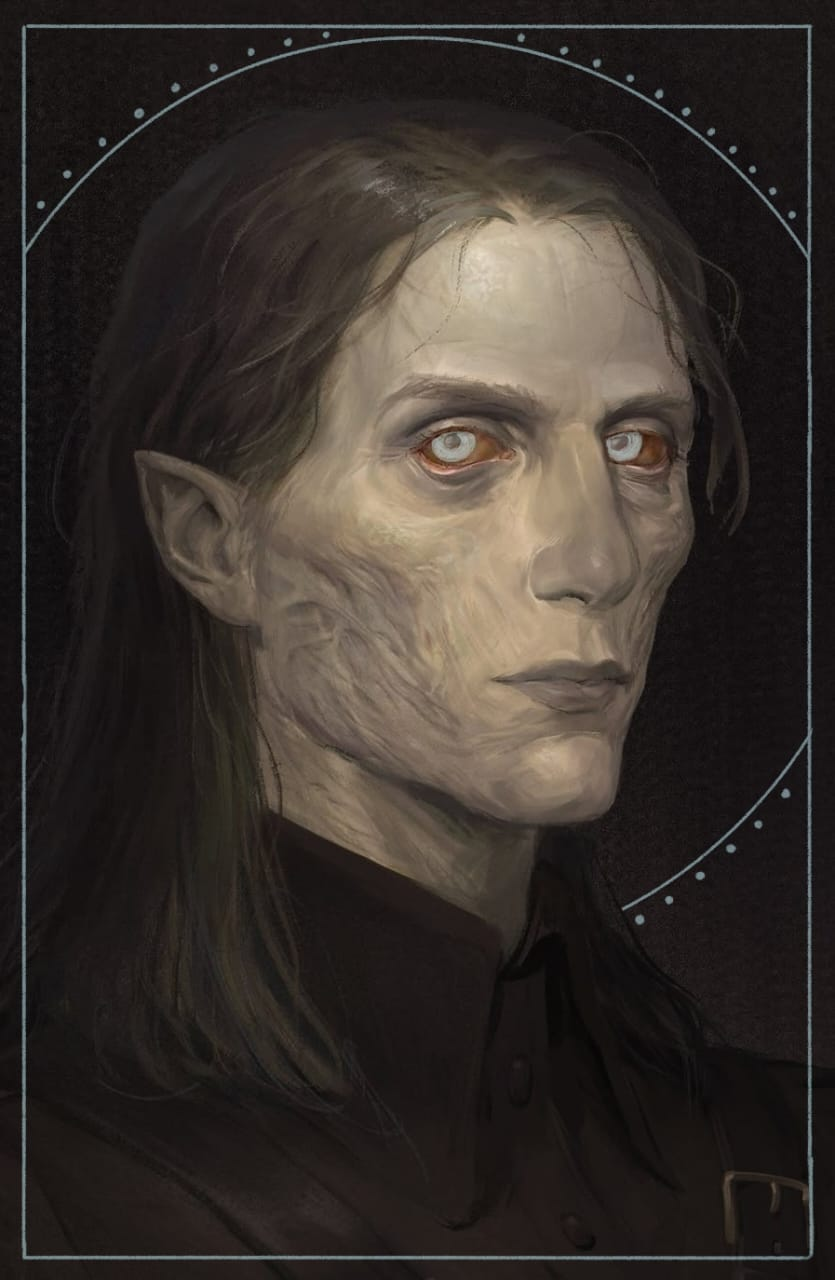
\includegraphics[width=0.22\textwidth]{Images/bat.jpeg}
\end{figure}

\begingroup
\DndSetThemeColor[PhbMauve]
\begin{DndSidebar}{Unholy Offspring}
\textit{The \textbf{Dhampir} are spawned from the cursed womb of a \textbf{Vampiric Matron}, a \textbf{consort to a Vampire Lord}. Often born out of wedlock, bastards to lesser men and dhampir.}
\end{DndSidebar}
\endgroup

\subsection{Chymaera}
The birth of twins aren't uncommon, but the rejoining of the souls within the womb very much is. Through scientific, necromantic or mutagenic interference, these beings born of humans show no physical difference, but harbour two souls. Often frightening parents into thinking their children are schizophrenic or possesed, these misunderstood children often end up lost or killed.
\textbf{Dual Mind. }You have advantage on all Wisdom saving throws.

\textbf{Mental Discipline. }You have resistance to psychic damage.


\textbf{Mind Link. } You can speak telepathically to any creature you can see, provided the creature is within a number of feet of you equal to 10 times your level. You don't need to share a language with the creature for it to understand your telepathic utterances, but the creature must be able to understand at least one language.
       

\textbf{Severed Spirits} Using the power of your other half you can either restore a level 1 spell slot 2 ki points or 1 specialty dice/resource up of a magical nature once every long rest for either yourself or a party member within 30 ft.

\subsection{Reborn}
Death isn’t always the end. The reborn exemplify this, being individuals who have died yet, somehow, still live. Some reborn exhibit the scars of fatal ends, their ashen flesh or bloodless veins making it clear that they’ve been touched by death. Other reborn are marvels of magic or science, being stitched together from disparate beings or bearing mysterious minds in manufactured bodies. Whatever their origins, reborn know a new life and seek experiences and answers all their own.


    \textbf{Ancestral Legacy. }If you replace a race with this lineage, you can keep the following elements of that race: any skill proficiencies you gained from it and any climbing, flying, or swimming speed you gained from it.
        If you don't keep any of those elements or you choose this lineage at character creation, you gain proficiency in two skills of your choice.

    \textbf{Deathless Nature.} You have escaped death, a fact represented by the following benefits:
        You have advantage on saving throws against disease and being poisoned, and you have resistance to poison damage.
        You have advantage on death saving throws.
        You don’t need to eat, drink, or breathe.
        You don’t need to sleep, and magic can’t put you to sleep. You can finish a long rest in 4 hours if you spend those hours in an inactive, motionless state, during which you retain consciousness.



   \textbf{ Knowledge from a Past Life.} You temporarily remember glimpses of the past, perhaps faded memories from ages ago or a previous life. When you make an ability check that uses a skill, you can roll a \textbf{d6} immediately after seeing the number on the \textbf{d20} and add the number on the \textbf{d6} to the check. You can use this feature a number of times equal to your proficiency bonus, and you regain all expended uses when you finish a long rest.

\begin{figure}[ht]
\centering
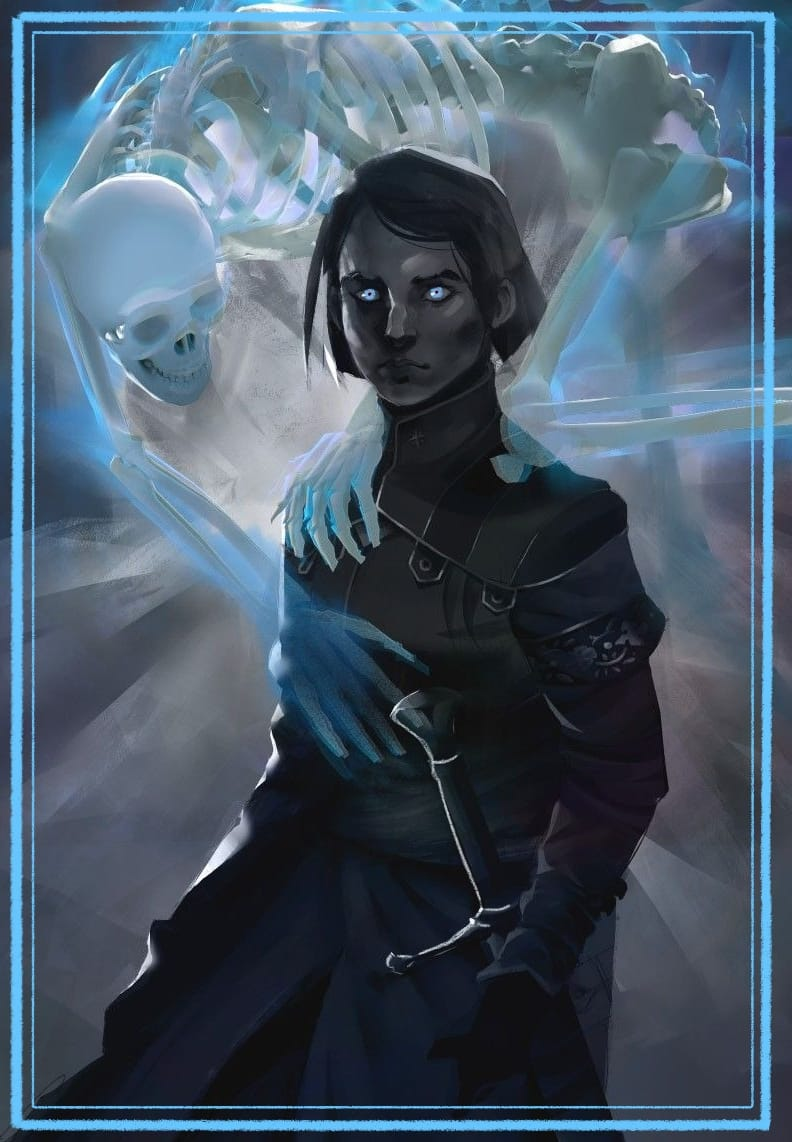
\includegraphics[width=0.228\textwidth]{Images/chym_possible.jpeg}

\includegraphics[width=0.22\textwidth]{Images/menari.jpeg}
\end{figure}

\begingroup
\DndSetThemeColor[PhbMauve]
\begin{DndSidebar}{Unholy Offspring}
\textit{The \textbf{Dhampir} are spawned from the cursed womb of a \textbf{Vampiric Matron}, a \textbf{consort to a Vampire Lord}. Often born out of wedlock, bastards to lesser men and dhampir.}
\end{DndSidebar}
\endgroup

\chapter{Religions}

\begin{figure}[H]
    \centering
    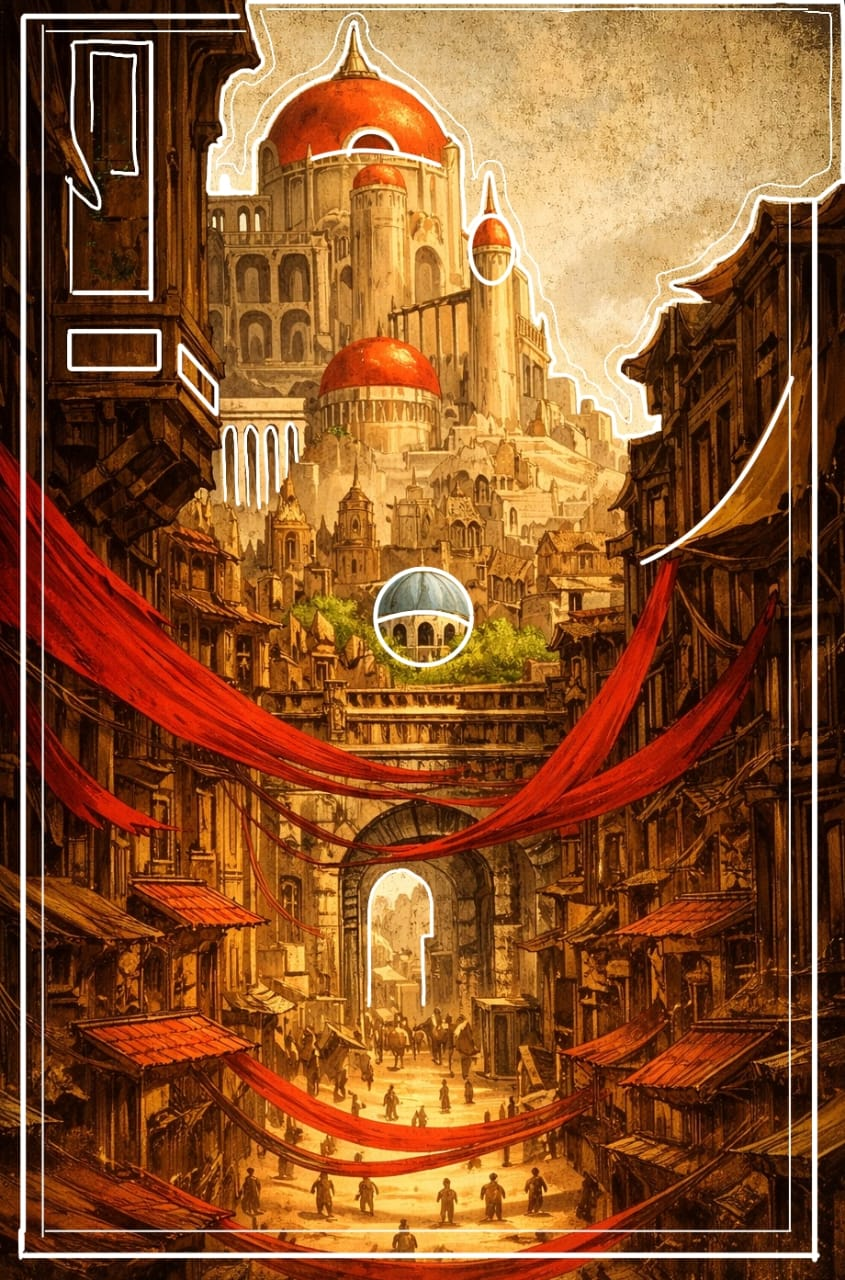
\includegraphics[width=0.75\linewidth]{Images/romulon.jpeg}
    \label{fig:placeholder}
\end{figure}

\begingroup
\DndSetThemeColor[PhbMauve]
\begin{DndSidebar}{Pillars of Eternity}
\textit{Streaked with golden pillars and domed roofs, \textbf{Romulon} is a vast and modern city.}
\end{DndSidebar}
\endgroup

\section{Alignment \& belief}

\DndDropCapLine{T}{}here are layers within layers when it comes to the religions found in this world,
however there are \textit{\textbf{pillars that support the foundations of the very structure of reality}}. Each main religion has a \textbf{\textit{unique domain}} tied to it, with divine influence exacted by \textit{few chosen clerics}.

\subsection{Gnocism}
%Lawful Good

The religion governed by the \textit{\textbf{Greater Will}} is known as Gnocism, the \textit{belief in a hidden, uncorrupted supreme being and a flawed \textbf{demiurge}} known as the \textit{\textbf{palm of creation}}, responsible for creating material reality. The \textit{\textbf{main church of Avaticana}} is centred in \textbf{Romulon}, city of the High Elves and serves as the \textit{political and religious hub} for the majority of the known world. The three sub sects of the Church is that of\textbf{ Apophystic Gnocism}, \textbf{Mystic Gnocism }and \textbf{Teleistic Gnocism}. Most folk tend to just serve the church without delving too deep into the theological aspect thereof. Its people are generally peaceful, however ancient \textit{holy wars} were fought quite recently against their greatest rivals the Vhaethiri, believers in \textbf{Aposiopism} and \textit{Her Web of Lies.}

\subsubsection{Religious Leader}
\textbf{The Pontifex, father Indorilius}, \textit{previously a humble Temple Knight}, is the current leader of this religious movement, elected at the \textit{\textbf{Conclave of the Chosen }}for his service in \textit{\textbf{the Crusade of Lies}}.

\subsection{Aposiopism}
%spiders and drow
%Lawful Evil


\subsubsection{Religious Leaders}


\begin{figure}[H]
\centering
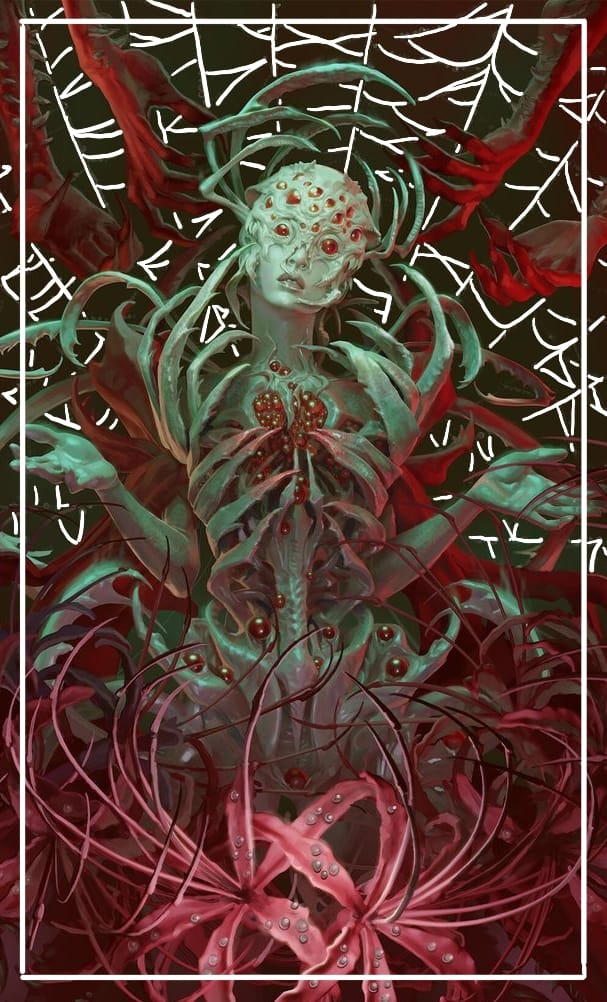
\includegraphics[width=0.22\textwidth]{Images/web.jpeg}
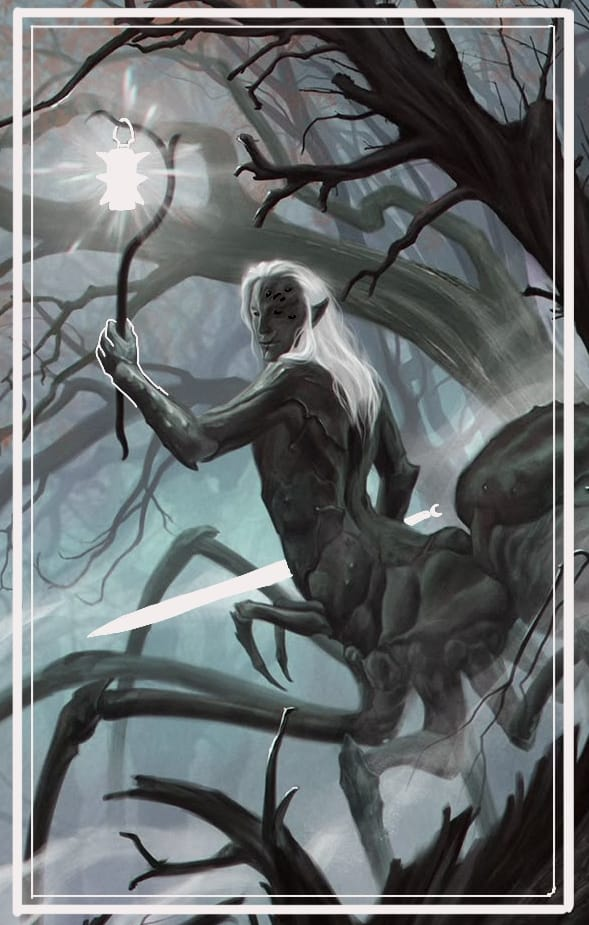
\includegraphics[width=0.232\textwidth]{Images/drider.jpeg}
\end{figure}

\subsection{Tar-Vasham}
%towers and Qunari
%Lawful Neutral

\subsection{Empyrealism}
%frenzied flame
%Chaotic Neutral

\begin{figure}[H]
    \centering
    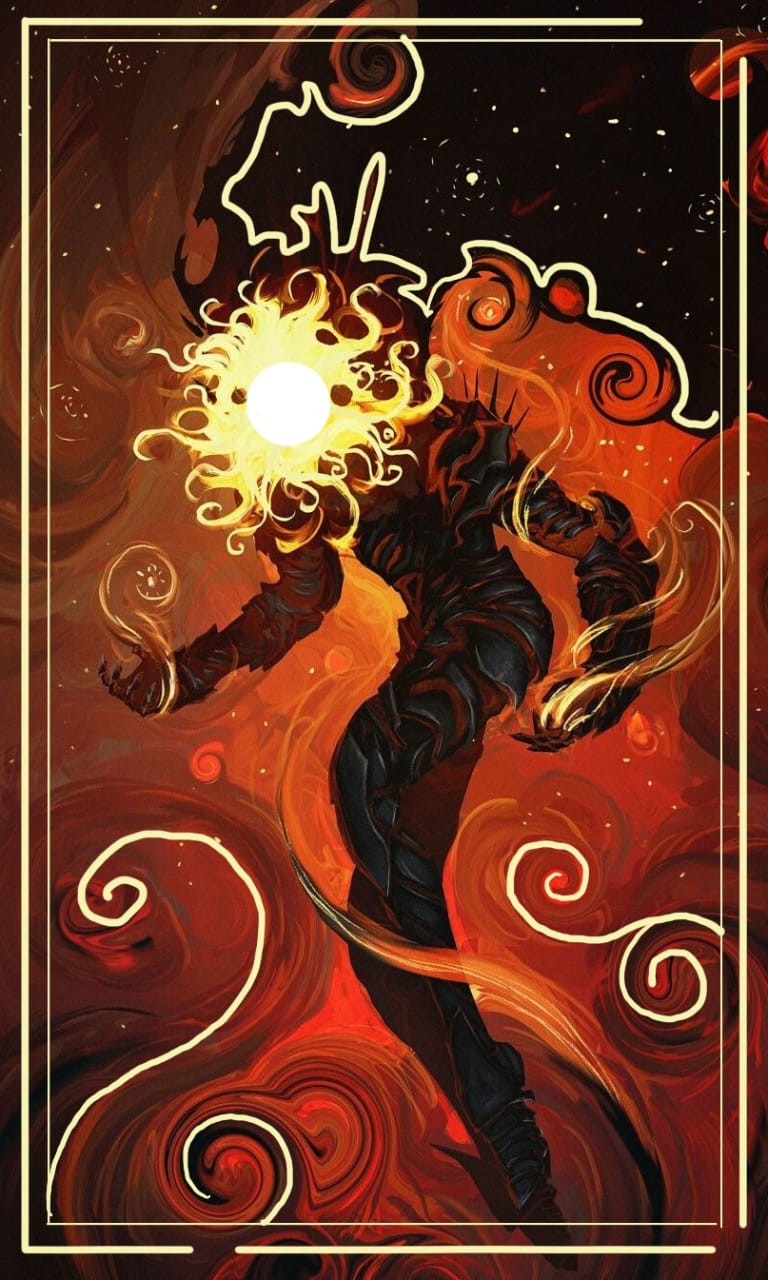
\includegraphics[width=0.71\linewidth]{Images/frenzy_inf.jpeg}
    \label{fig:placeholder}
\end{figure}

\subsection{Viridism}
%verdant oath, wood elves and nature
%Chaotic Good

\subsection{Miasmism} 
%Ruinous Rot
%Chaotic Evil

\begin{figure}[H]
    \centering
    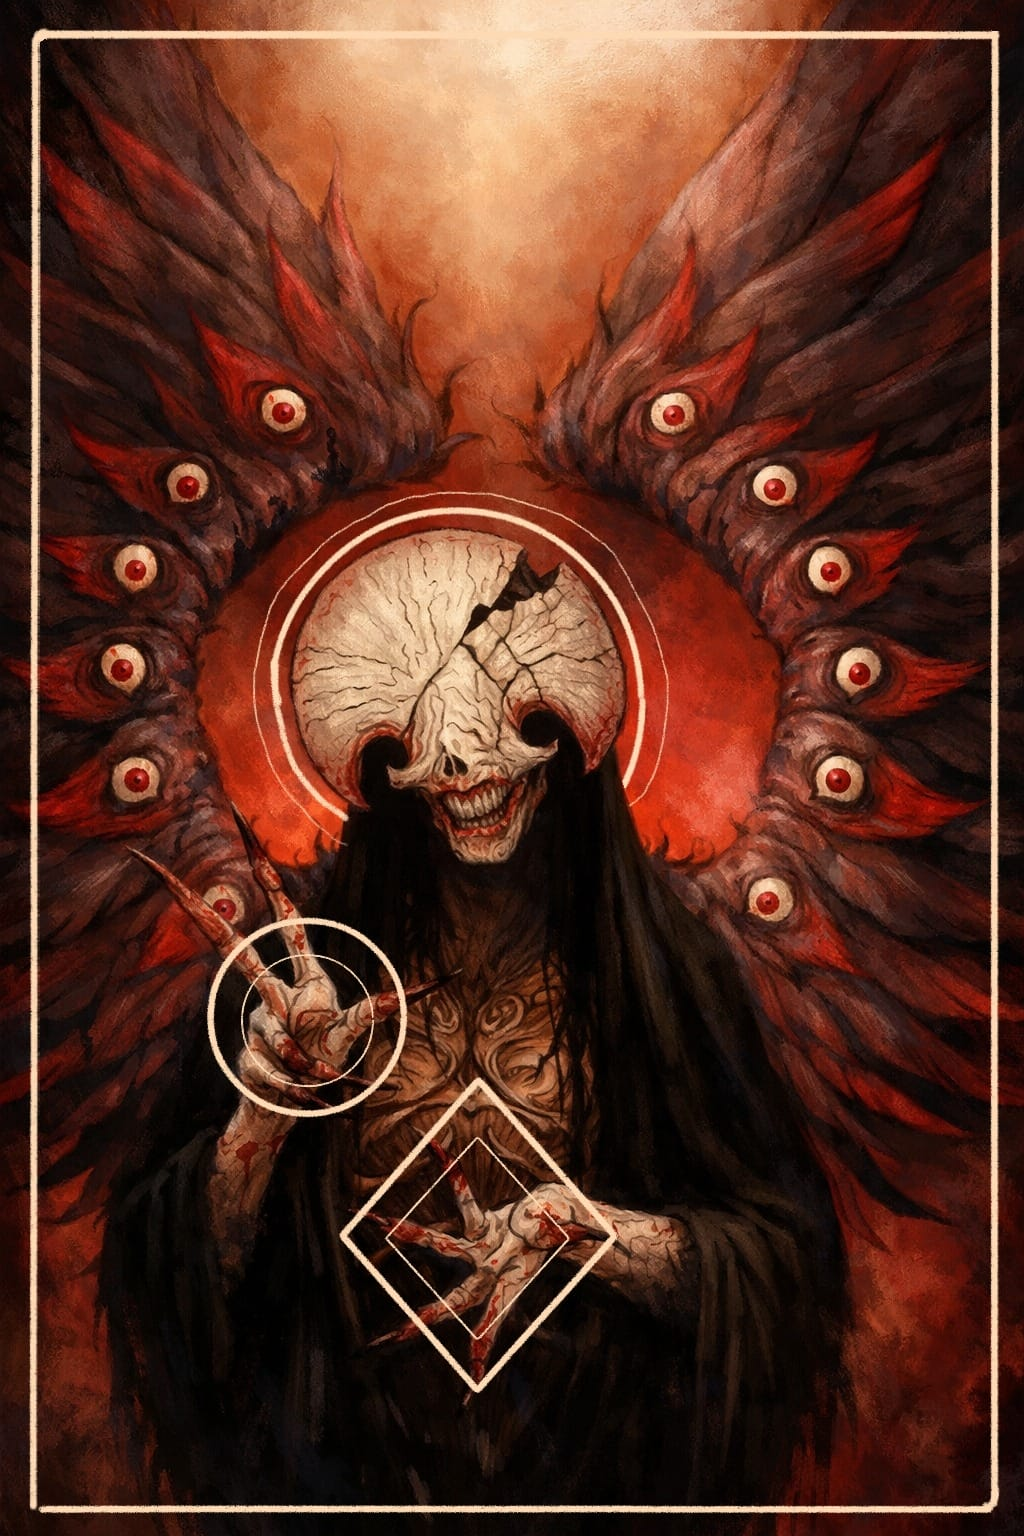
\includegraphics[width=0.75\linewidth]{Images/rotten_one.jpeg}
    \label{fig:placeholder}
\end{figure}

\subsection{}
%
%Neutral Good

\subsection{Proditism}
%Dread Wolf, orcs.
%Neutral Evil

\begin{figure}[H]
    \centering
    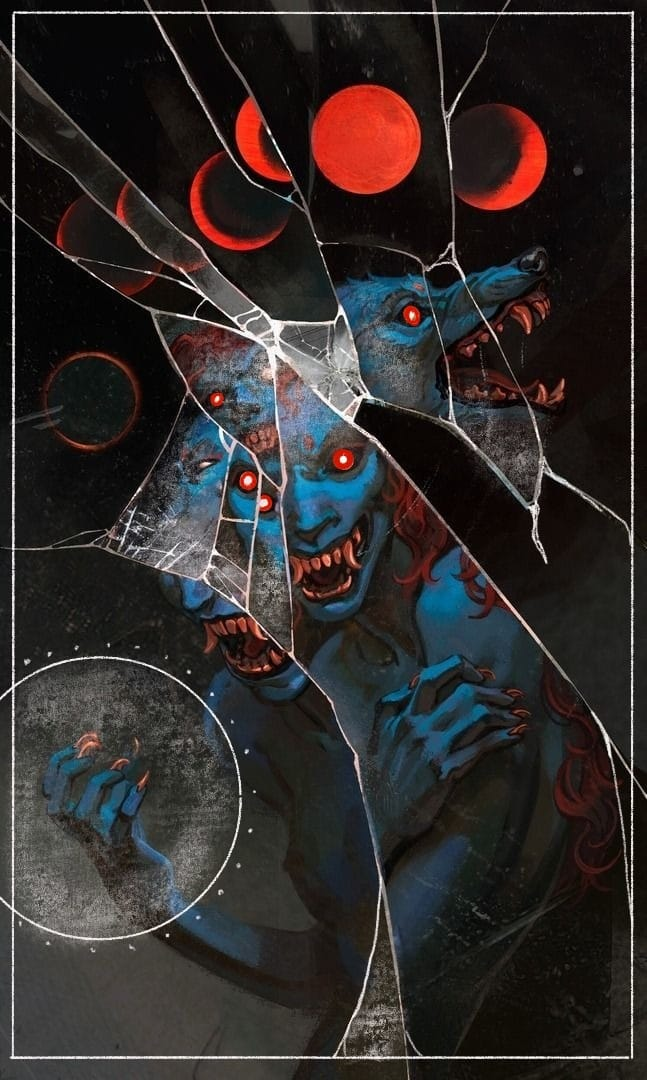
\includegraphics[width=0.7\linewidth]{Images/wolf.jpeg}
    \label{fig:placeholder}
\end{figure}

\chapter{Effects \& Afflictions}

\section{Diseases}
\DndDropCapLine{Y}{}ou find yourself in a world rife with divine curses, man-made disease and magic anomalies, some of them are listed here, beware to not contract theml for it may spell your end.

\begin{figure}[H]
    \centering
    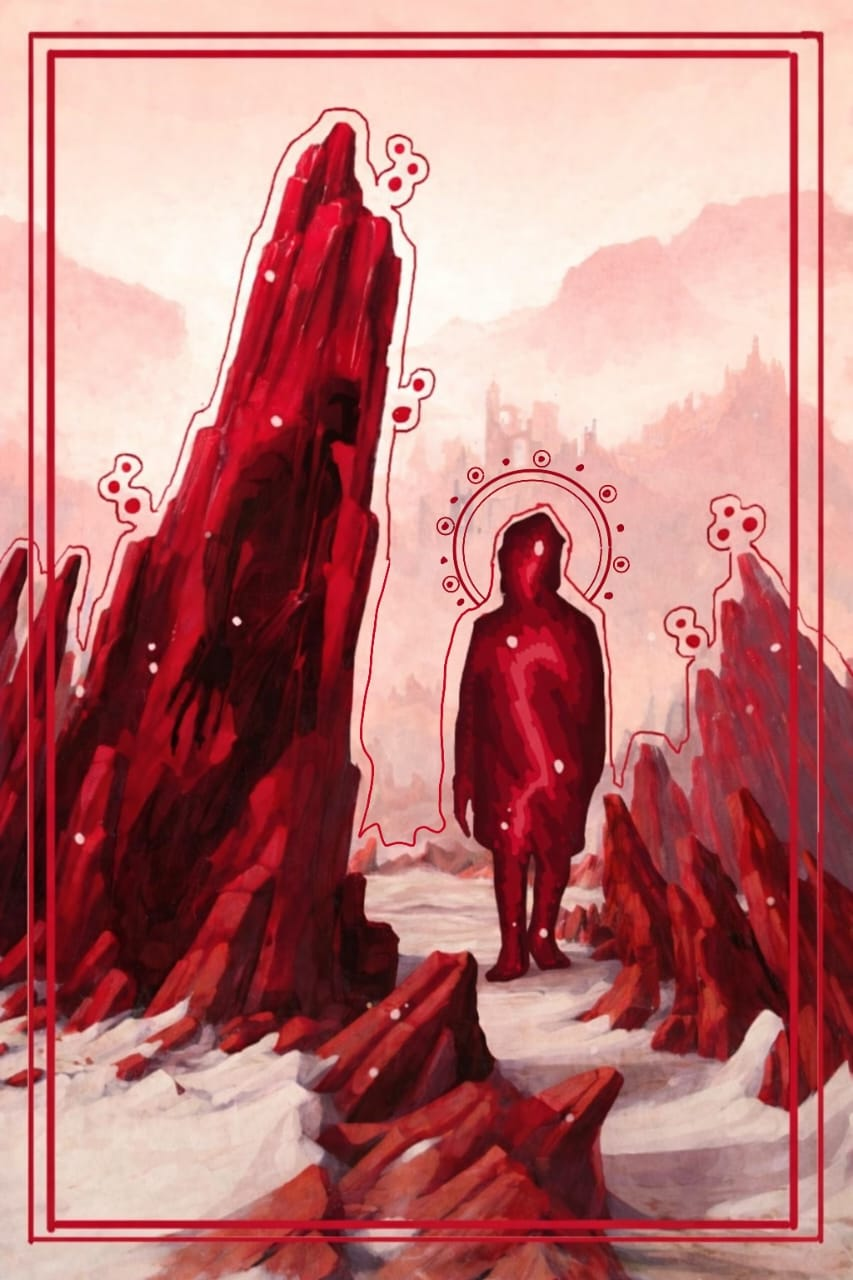
\includegraphics[width=0.6\linewidth]{Images/red_lyr.jpeg}
    \label{fig:placeholder}
\end{figure}

\begingroup
\DndSetThemeColor[PhbMauve]
\begin{DndSidebar}{Pillars of Eternity}
\textit{Streaked with golden pillars and domed roofs, \textbf{Romulon} is a vast and modern city.}
\end{DndSidebar}
\endgroup

\subsection{Lyrium Drawbacks}
\label{main:lyrium}\appendixlink{lyrium}{Appendix IV}{Red Lyrium Enemies}
Blue Lyrium, a magical stimulant used by mages, sorcerers, paladins, eldritch knights etc. is used to empower their spellcasting abilities, in the case of the abyssal tieflings, outright removing the need for any material components, with the exception of warlocks and clerics as their power isn't innate. Red Lyrium, a poor attempt at an artificial substitute to Blue Lyrium, is a chaotic growth of bright ruby crystals found underground in the deep roads. A creation of the Dwerfen Gemmists, abandoned and sealed due to its failed, corrupting behaviour. The Blue Lyrium trade however has provided to be quite lucrative and many mercenary companies and smugglers seek to profit from this dangerous pharmaceutical.

\DndSpellHeader%
  {Rubrilyriasis}
  {Special affliction}
  {Varies (see Exposure)}
  {Self (proximity) or touch}
  {Active Red Lyrium Crystals}
  {Until removed from exposure; progression is permanent}
\textbf{Ambient Exposure (Mind).} If you spend more than \textit{10 minutes near red lyrium}, make a Willpower (Self-Discipline) test (DC 11) or begin hearing \textit{Calling-like voices} urging you to ingest or physically contact red lyrium. Repeat this test each hour you remain near it. Each failure increases the DC of subsequent tests by +2. If you remain away from red lyrium for 3 consecutive hours, the DC resets to 11.

\textbf{Physical Exposure (Body).} If you are physically exposed to red lyrium, make a Constitution (Stamina) test (DC 11). Each failure increases the DC of subsequent tests by +2.

\textbf{Physical Failure Track.} On the 1st failed Constitution test, your skin takes on a reddish hue and you crave more red lyrium. On the 2nd failed test, you grow small red-lyrium nodules and begin to hunch and deform. On the 3rd failed test, you transform into a Red \textbf{Lyrium Horror, Red Lyrium Shadow, or Red Lyrium Behemoth.} On the 4th failed test, you die, overgrown with red lyrium, leaving crystals growing from your fallen form.

\textbf{Cure.} No cure is known; red lyrium contact is treated as an inevitable death sentence. A possible cure could include a \textit{limited or full wish spell}.

\begin{figure}[H]
    \centering
    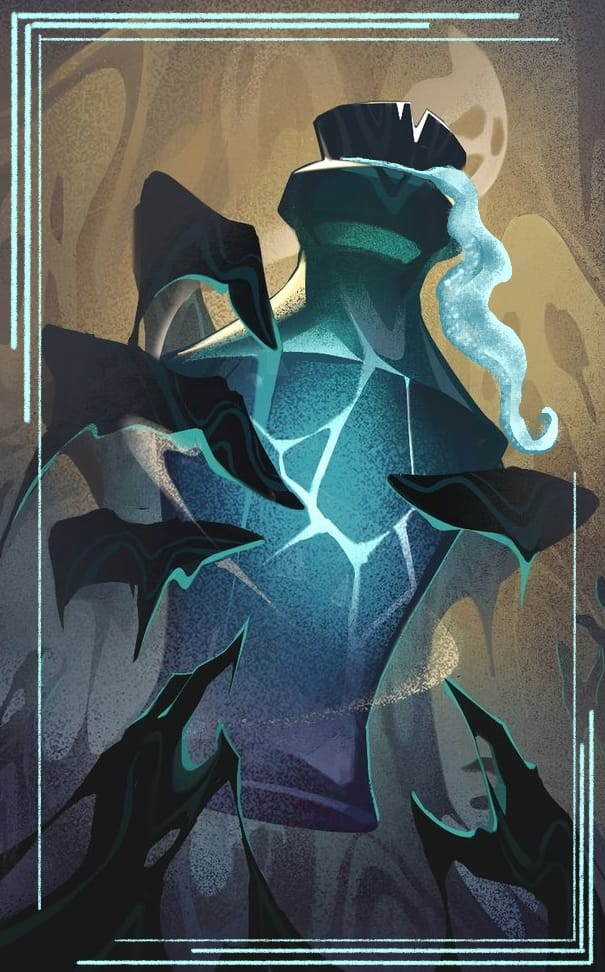
\includegraphics[width=0.6\linewidth]{Images/lyrium.jpeg}
    \label{fig:placeholder}
\end{figure}

\begingroup
\DndSetThemeColor[PhbMauve]
\begin{DndSidebar}{Pillars of Eternity}
\textit{Streaked with golden pillars and domed roofs, \textbf{Romulon} is a vast and modern city.}
\end{DndSidebar}
\endgroup

\DndSpellHeader%
  {Caeruleolyriasis}
  {Special affliction (blue lyrium withdrawal)}
  {1 hour (escalates)}
  {Self}
  {None}
  {Until cured}
When you are separated from a steady supply of \textbf{blue lyrium} (or attempt to stop using it), you suffer \textbf{Caeruleolyriasis} (blue-lyrium withdrawal). While afflicted, you experience fatigue, forgetfulness, a gnawing thirst, and cold hands. As the hunger deepens, paranoia and obsession intensify; you may struggle to separate memory from the present, or waking from dream.

\textbf{Craving Spiral.} At the end of each long rest without blue lyrium, make a Wisdom saving throw (DC 11). On a failure, the DC increases by +2 for subsequent saves until you either consume blue lyrium or complete 3 consecutive long rests without failing. On your \textbf{third failure}, you must use your next available downtime or opportunity to seek blue lyrium, prioritizing it over other goals unless doing so would cause immediate, obvious death.

\textbf{Withdrawal Side-Effect.} Each time you fail the Wisdom saving throw for \textbf{Craving Spiral}, roll a d8 on your withdrawal side-effect table and apply the result until you finish a long rest (or longer, if the table says so).

\textbf{Mental Fog.} While Caeruleolyriasis is active, you have disadvantage on checks made to recall information, track time, or resist intimidation and manipulation that promises relief.

\textbf{Fade Echoes (Full-casters).} If you can cast spells, on a failed save you also hear indistinct voices and suffer brief dizzy spells; on a success, these symptoms lessen after a long rest. Unlike paladins or eldritch knights, mages may recover from the adverse effects with rest and abstinence, at the GM's discretion.

\textbf{Cure.} A healer's regimen, supervised withdrawal, or powerful restorative magic may end Caeruleolyriasis. In settings where lyrium dependence is considered irreversible, treatment only manages symptoms rather than curing them.

\begin{DndTable}[color=PhbLightCyan]{cX}
  \textbf{d6} & \textbf{Withdrawal Side-Effect} \\
  1 & \textbf{Dermal Luminescence.} You shed dim light 5 ft. and have disadvantage on Dexterity (Stealth).\\
  2 & \textbf{Arcano-Dyslexia.} For 1 hour, you must succeed on a DC 12 Intelligence check to read normally. \\
  3 & \textbf{Perceptual Desync.} You have disadvantage on initiative rolls.\\
  4 & \textbf{Fine-Motor Tremor.} You have disadvantage on Dexterity checks made with tools.\\
  5 & \textbf{Scar Irradiation.} You can’t gain temporary hit points.\\
  6 & \textbf{Resistance.} You resist additional withdrawal effects.\\
\end{DndTable}

\begin{figure}[H]
    \centering
    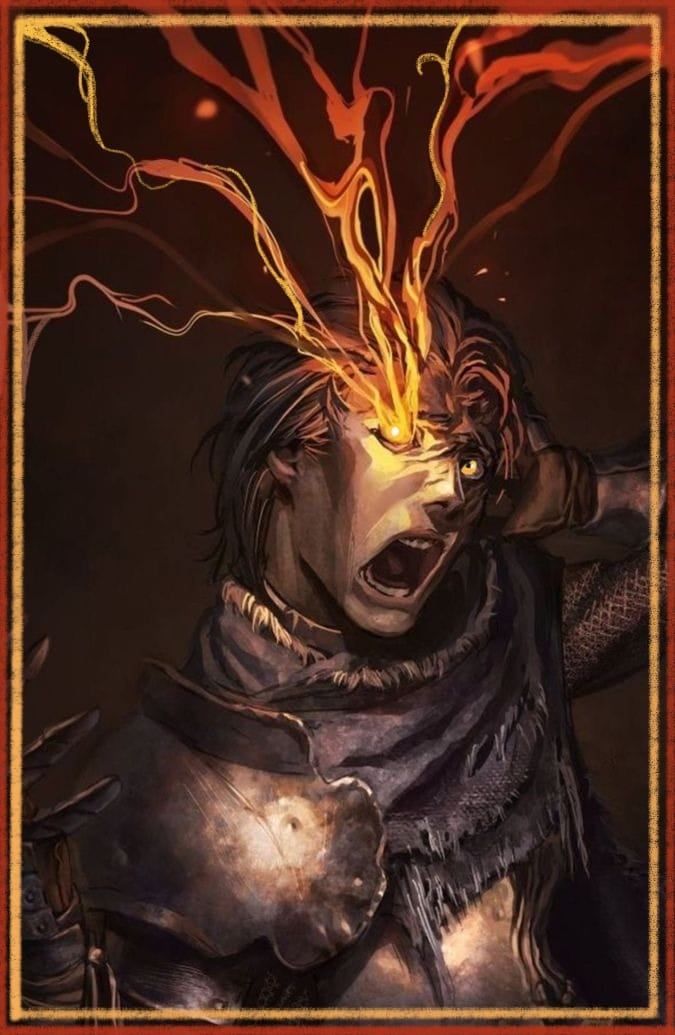
\includegraphics[width=0.6\linewidth]{Images/fr_fl.jpeg}
    \label{fig:placeholder}
\end{figure}

\begingroup
\DndSetThemeColor[PhbMauve]
\begin{DndSidebar}{Pillars of Eternity}
\textit{Streaked with golden pillars and domed roofs, \textbf{Romulon} is a vast and modern city.}
\end{DndSidebar}
\endgroup

\subsection{Purgeflame}
\label{main:purgeflame}\appendixlink{purgeflame}{Appendix I}{Purgeflame Spells}

flavour text

\DndSpellHeader%
  {Empyrosis}
  {Special affliction (the Purgeflame)}
  {Ongoing (slow progression)}
  {Self}
  {None}
  {Until cured (or irreversible)}
Empyrosis is the Purgeflame behind the eyes: a bright, cleansing lie that rewards surrender. It does not spread by time alone. It spreads by \emph{agreement}.

\textbf{Ember Marks.} Empyrosis is tracked with \textbf{Ember Marks} (0--6). You gain Ember Marks primarily by \textbf{giving in} and using Empyrosis gifts. You may also gain 1 Ember Mark at the GM's discretion after major exposure to the Purgeflame.

\textbf{Feeding the Purgeflame.} Each time you use an Empyrosis gift, you gain \textbf{1 Ember Mark} \emph{after the effect resolves}. If the gift caused a creature to trigger Madness Threshold, you gain \textbf{1 additional Ember Mark}.

\textbf{Slow Drift.} At the end of each \textbf{7 days} in which you did \emph{not} use an Empyrosis gift, reduce your Ember Marks by \textbf{1} (minimum 0). This represents the Purgeflame cooling when you refuse it.

\textbf{Point of No Return.} At \textbf{6 Ember Marks}, Empyrosis becomes \textbf{Irreversible}. Your Ember Marks can no longer be reduced by any means, and you cannot be cured. You keep all unlocked gifts, but you are forever considered \emph{touched} by the Purgeflame.

\textbf{Madness Threshold.} When you gain an Ember Mark that brings you to \textbf{3 or more}, you become vulnerable to flare-ups. Whenever you roll initiative, make a Wisdom saving throw (DC 11 + your Ember Marks). On a failure, you become \textbf{Mad}. While Mad, you take \textbf{fire damage equal to twice your CR (or level, minimum 1)} at the start of each of your turns. This damage cannot be reduced or ignored in any way. When you become Mad, you are \textbf{stunned} until the end of your next turn, then the Madness ends.

\textbf{Staged Gifts (Once per Long Rest).} As your Ember Marks rise, Empyrosis unlocks gifts. Each gift can be used \textbf{once per long rest}. Using any gift feeds the Purgeflame as described above.

\textbf{Stage I (Ember scars 1+):} \emph{Purgeflare Cone}

\textbf{Stage II (Ember scars 2+):} \emph{Cry of Shabriel}

\textbf{Stage III (Ember scars 3+):} \emph{Unendurable Purge}

\textbf{Stage IV (Ember scars 4+):} \emph{Inescapable Purge}

\textbf{Stage V (Ember scars 5+):} \emph{Purging Inferno}

\textbf{Cure (Unique).} Empyrosis can be cured only by bathing in the waters of the \textbf{Lazerian Oasis}. A full immersion for at least 10 minutes during a long rest removes all Ember Marks and ends Empyrosis \emph{if and only if} you have not reached the Point of No Return.

\begin{figure}[H]
    \centering
    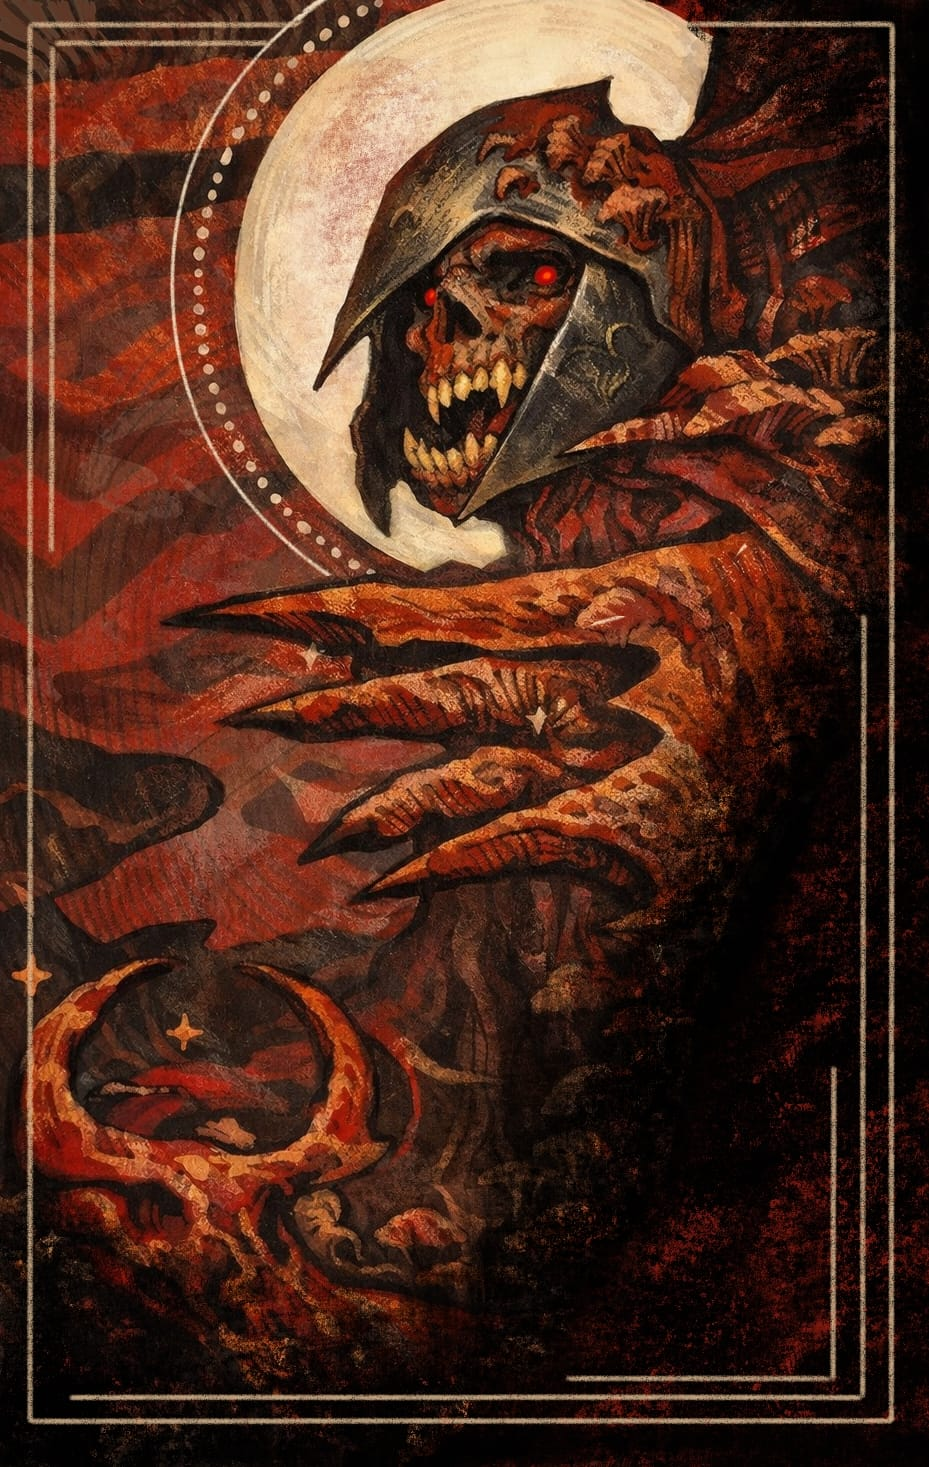
\includegraphics[width=0.6\linewidth]{Images/rot.jpeg}
    \label{fig:placeholder}
\end{figure}

\begingroup
\DndSetThemeColor[PhbMauve]
\begin{DndSidebar}{Pillars of Eternity}
\textit{Streaked with golden pillars and domed roofs, \textbf{Romulon} is a vast and modern city.}
\end{DndSidebar}
\endgroup

\medskip

\subsection{Red Rot}
\label{main:redrot}\appendixlink{redrot}{Appendix II}{Red Rot Spells}

It acts as an incurable, infectious disease that decays the bodies and minds of living things. The manifestation of the outer deity of rot, this 

\DndSpellHeader%
  {Apoptosia}
  {Special affliction (Red Rot)}
  {Ongoing (slow progression)}
  {Self}
  {Rot-infested Material}
  {Until cured (or irreversible)}
Apoptosia is a strain of the \textbf{Red Rot}: a plague-rot that consumes flesh, spoils vitality, and flowers in damp, blighted places. It spreads slowly, but it tightens fastest when you \emph{use} it.

\textbf{Rotwound.} Track Apoptosia with \textbf{Rotwound} (0--5).

\textbf{Contracting the Blight.} When you suffer major exposure to the Red Rot (wading in rot, breathing spores, being struck by a rot attack), make a Constitution saving throw (DC 12). On a failure, gain \textbf{1 Rotwound}.

\textbf{Feeding the Blight.} Each time you use a \textbf{Plagueboon}, you gain \textbf{1 Rotwound} after the effect resolves. This is the core rule: \emph{power strengthens the grip}.

\textbf{Rotting Pulse.} Whenever you gain a Rotwound, you take \textbf{2d6 necrotic damage}. While you have \textbf{3+ Rotwound}, you take \textbf{1d4 necrotic damage} at the start of each of your turns.

\textbf{Odd-Stage Boons.} At Rotwound \textbf{1, 3, and 5}, you gain a boon.

\textbf{Point of No Return.} At \textbf{Rotwound 4}, Apoptosia becomes \textbf{Irreversible}. Your Rotwound can no longer be reduced, and you cannot be cured by any means.

\textbf{Cure and Mitigation (Before 4).} Before Rotwound 4, Apoptosia can be cured or reduced by powerful cleansing rites and remedies at the GM's discretion.

\medskip

\textbf{Stage I (Rotwound 1).} \textbf{Boon: Spore-Sense.} You gain advantage on Perception checks to detect diseased, blighted, or poisonous creatures and terrain.
You unlock the Plagueboon \emph{Touch of Decay} (Once per Long Rest).

\textbf{Stage II (Rotwound 2).} Fever-dreams gnaw your rest. You have disadvantage on checks to resist exhaustion caused by sleeplessness or forced marches.

\textbf{Stage III (Rotwound 3).} \textbf{Boon: Blight Exultation.} Once on each of your turns, when you deal necrotic or acid damage, add \textbf{+1d4} to one damage roll.
You unlock the Plagueboon \emph{Carrion-Breath} (Once per Long Rest).

\textbf{Stage IV (Rotwound 4).} \textbf{Irreversible.} Your body begins to warp with subtle ways as the blight becomes you. You have disadvantage on Wisdom saving throws against fear and charm, but advantage on constitution saves against being poisoned.

\textbf{Stage V (Rotwound 5).} \textbf{Boon: Crown of Bloom.} You gain resistance to \textit{necrotic damage}.
You unlock the Plagueboon \emph{Abyssal Bloom} (Once per Long Rest).

\subsection{Lycanthropy}
\label{main:lycanthropy}\appendixlink{lycanthropy}{Appendix III}{Carlislean Lycanthrope (Monster Class)}

Carlisle was a wretched, fainthearted man of no renown, who wearied of being kicked aside and went begging for strength. In the old wood he found the Dread Wolf, and took its bargain: stout sinew and a predator’s bite, in return for a heart that would sooner turn coat than stand fast. The curse didn’t end with Carlisle, it clung to teeth and bloodlines, spreading wherever desperate people wanted strength more than they wanted to stay themselves.

\DndSpellHeader%
  {Canis Hysteria}
  {Special curse-disease (Carlislean strain)}
  {Ongoing (stage progression)}
  {Self}
  {Physical Wound caused by a werewolf}
  {Until cured, transformed, or sealed}

\textbf{Origin.} The first werewolf was \textbf{Carlisle}, a human cursed by the \textbf{Dread Wolf}, a neutral evil outer god of \textbf{treachery, tyranny, and ambition}. All Carlislean werewolves descend from this single curse-line.

\textbf{Stages.} Track the curse from \textbf{Stage 1} to \textbf{Stage 5}. Stages 1--3 progress like a disease. Stages 4--5 are metamorphosis.

\textbf{Stage Advancement (1--3).} After each \textbf{long rest} while infected, make a Constitution saving throw (DC 12). On a failure, advance by 1 stage (maximum Stage 3 by disease alone).

\textbf{Human Hearts (3 $\rightarrow$ 5).} Eating a \emph{fresh humanoid heart} cannot advance you from Stage 1 to Stage 3. It \textbf{only} advances you from \textbf{Stage 3 to Stage 5} (one stage per heart, maximum one heart per long rest).

\textbf{Coronation of the Wolf (Stage 5 Seal).} To become a \textbf{full werewolf}, you must \textbf{kill another werewolf and feast on its heart}. If you are Stage 3 or higher, doing so immediately advances you to \textbf{Stage 5} and you become \textbf{sealed}.

\textbf{Full Moon Trial.} On each \textbf{full moon}, you transform at dusk and must succeed on a Wisdom saving throw (DC 14 + your current stage) or be compelled to hunt a heart to \emph{quicken or solidify} the curse. 

\textbf{Temporary Transformation (Stages 1--3).} During the full moon you may transform into a hybrid form. While transformed, you have:
\begin{itemize}
\item \textbf{Multiattack} (2 attacks).
\item \textbf{Resistance} to bludgeoning, piercing, and slashing damage from \textbf{nonmagical, nonsilver} sources.
\item \textbf{Bite (Healing).} Once per turn, when you hit with your bite, you regain hit points equal to the damage dealt.
\end{itemize}

\textbf{Stage 1: Keen Flesh (Human Form).}
\begin{itemize}
\item \textbf{Predator Senses.} Advantage on Perception checks relying on smell, hearing, or sight.
\end{itemize}

\textbf{Stage 2: Raw Hunger (Human Form).}
\begin{itemize}
\item \textbf{Craving.} If you begin a long rest without having eaten \textbf{fresh raw meat} that day, you start the rest with \textbf{1 level of exhaustion} (removed if you eat raw meat before the rest ends).
\end{itemize}

\textbf{Stage 3: Waxing Madness (Human Form).}
\begin{itemize}
\item \textbf{Moon-Pull.} During the \textbf{three nights leading up to the full moon}, you have disadvantage on Wisdom and Charisma saving throws.
\item \textbf{Threshold.} Disease progression stops here; only hearts (or the Coronation) push you further.
\end{itemize}

\textbf{Stage 4: Permanent Hybrid (Point of No Return).}
From this stage onward you are always partly changed: heavier musculature, more hair, sharper teeth, and a predator's stare. This is the \textbf{point of no return}; the curse cannot be cured by ordinary means.
\begin{itemize}
\item \textbf{Hardened Frame.} Strength +1.
\item \textbf{Magical Darkvision.} Darkvision 60 ft (or +30 ft if you already have it).
\end{itemize}

\textbf{Stage 5: Class Overwrite.} When you reach Stage 5, you gain levels equal to your current level of the \textbf{Carlislean Lycanthrope} monster class as though you were a \textbf{Gestalt character}. If you were\textit{ already a Gestalt character}, you\textit{ appropriately replace one of your current classes}.
\begin{figure}[H]
\centering
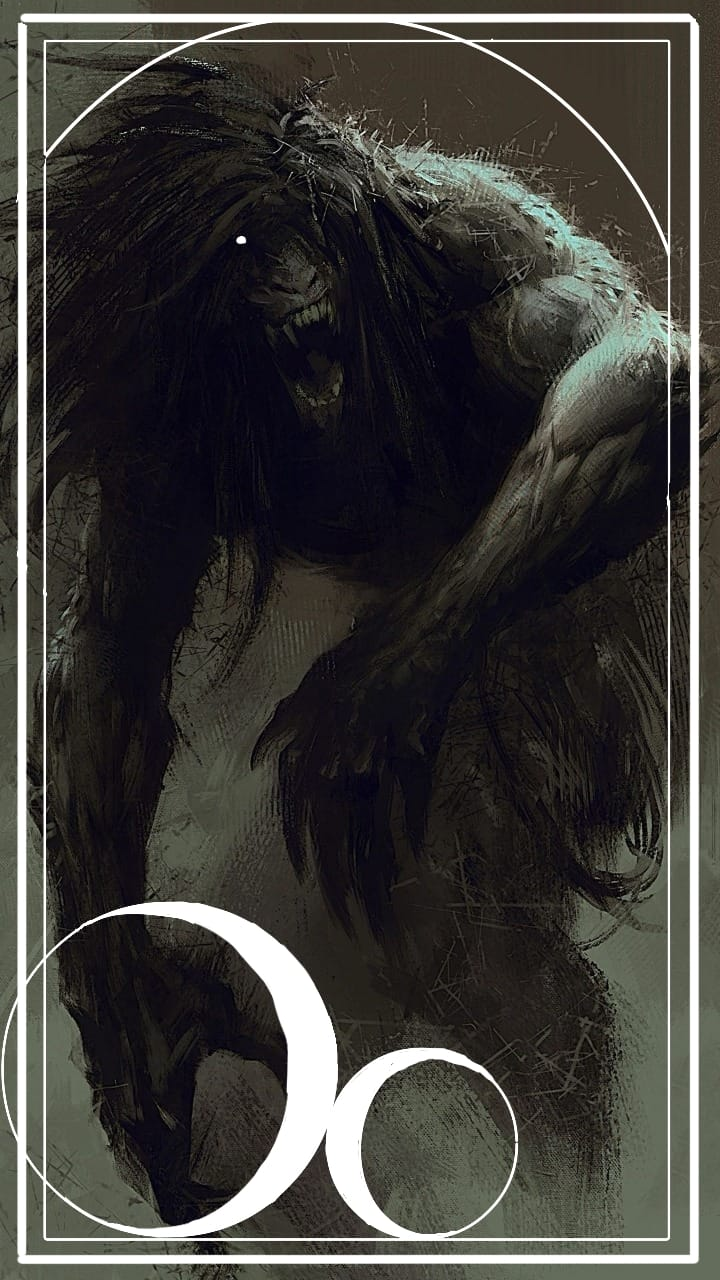
\includegraphics[width=0.2\textwidth]{Images/Werwulf.jpeg}
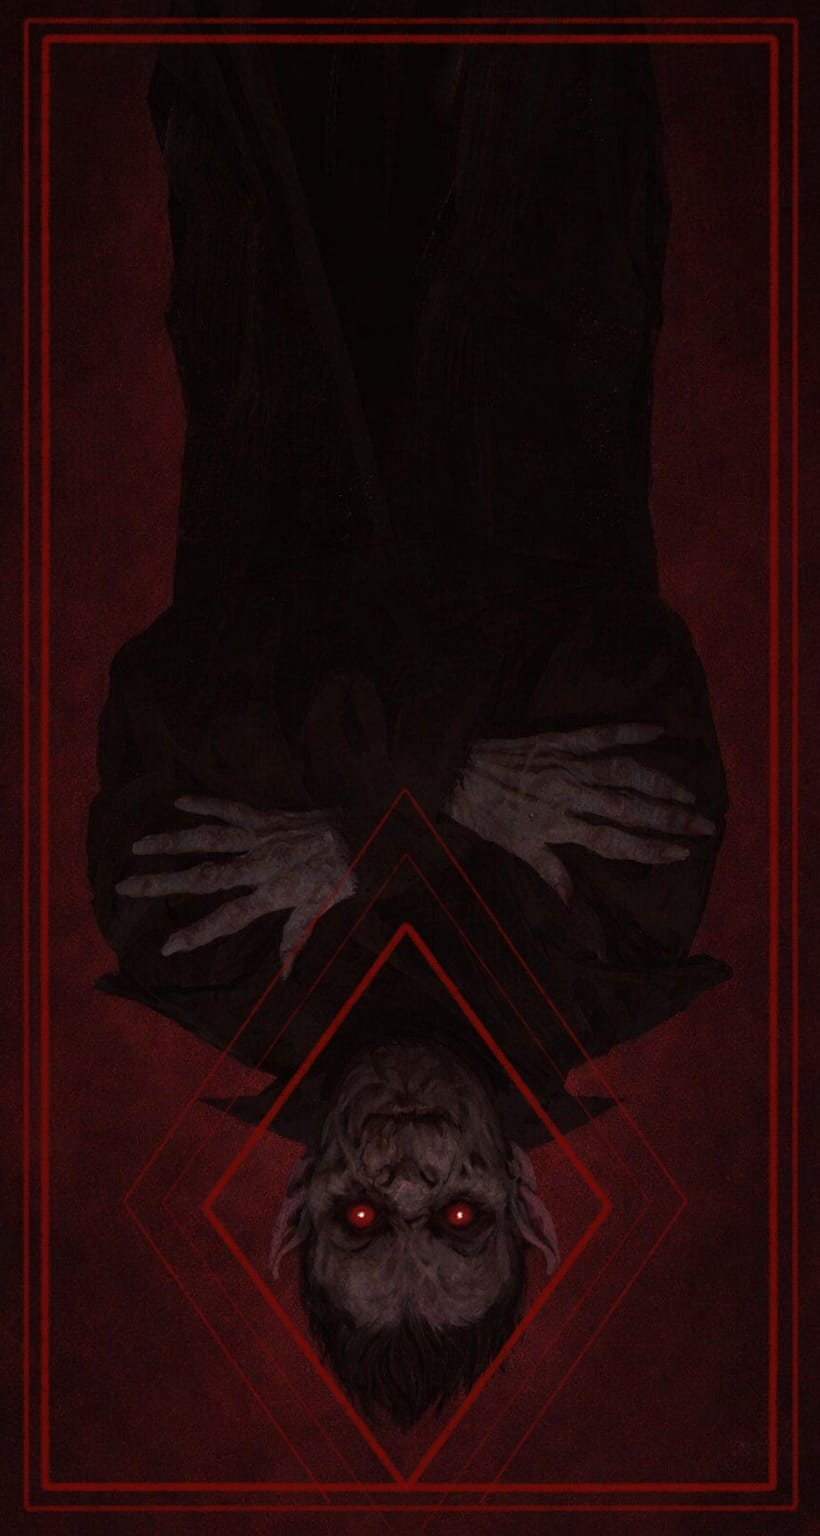
\includegraphics[width=0.19\textwidth]{Images/VAMP.jpeg}
\end{figure}

\begingroup
\DndSetThemeColor[PhbMauve]
\begin{DndSidebar}{Pillars of Eternity}
\textit{Streaked with golden pillars and domed roofs, \textbf{Romulon} is a vast and modern city.}
\end{DndSidebar}
\endgroup

\subsection{Dhampirism}

Dhampirs stand between life and death, endlessly tested by vicious hunger. Most inherit the condition through a vampiric bloodline, but it can also arise when a mortal \textbf{drinks a vampire's blood} and survives the taste.

\DndSpellHeader%
  {Sanguinare Dhampiris}
  {Special affliction}
  {Slow (stage-based)}
  {Self}
  {M (vampire blood, consumed)}
  {Until completed}

\textbf{Strain (Blood-Determined).} Your strain is determined by the \textbf{vampire blood} you consumed. You do not choose it.
\begin{itemize}
\item \textbf{Crystalline.} Iridescent and brittle-skinned; (\emph{Brittle Bones} manifests at Stage 3.)
\item \textbf{Chiropterine.} Bat-like and hairy; heightened awareness and keen reflexes. (\emph{Sunlight Sensitivity} manifests at Stage 3.)
\end{itemize}

\subsubsection{Progression:}
This is a light transformation. After meaningful exposure (GM discretion), such as consuming vampire blood, surviving a vampire's bite, or repeated feeding, make a Constitution saving throw (DC 12). On a failure, advance 1 stage (maximum Stage 3). On a success, you do not advance and take 3d6 necrotic damage as your body rejects the cursed blood.

\medskip

\textbf{Stage 1: Blood-Echo.}
Your body remembers the taste of death, and your senses sharpen.
\begin{itemize}
\item \textbf{Heightened Senses.} You gain advantage on Wisdom (Perception) checks.
\end{itemize}

\textbf{Stage 2: Half-Death.}
The change becomes visible: pallor, sharpened features, and a predatory stillness.
\begin{itemize}
\item \textbf{Darkvision.} You gain darkvision out to 60 feet.
\item \textbf{Life-Draining Bite.} You gain a bite attack that deals \textbf{2d4} damage and heals you for the damage dealt. This bite's damage becomes \textbf{2d6} at character level 4, \textbf{2d8} at level 8, and \textbf{2d10} at level 12.
\item \textbf{Strain Trait (emerges).}
\begin{itemize}
\item \textbf{Crystalline: Tough.} You gain the benefits of the feat: \textbf{tough} and \textbf{resistance to non-magical bludgeoning, piercing and slashing damage.}
\item \textbf{Chiropterine: Dread Ambusher.} You gain a \textbf{dread ambusher} feature from \textbf{Gloomstalker Rangers}.
\end{itemize}
\end{itemize}

\textbf{Stage 3: True Dhampir (Strain Weakness Manifests).}
You are now fully dhampir; hunger is no longer a symptom but the rest of your undead life.
\begin{itemize}
\item \textbf{Strain Weakness.}
\begin{itemize}
\item \textbf{Crystalline: Brittle Bones.} You become vulnerable to thunder damage.
\item \textbf{Chiropterine: Sunlight Sensitivity.} While in sunlight, you have disadvantage on attack rolls and on Wisdom (Perception) checks that rely on sight and gain vulnerability to radiant damage.
\end{itemize}
\end{itemize}

\subsection{Vampirism}

Vampires are cursed creatures of the night, spawn of the two original vampires. A vampire's bite can seed a living body with a cursed strain. The strain does not advance by chance or fortitude, but by \textbf{indulgence}: the curse grows stronger each time you feed it what it truly wants.

\DndSpellHeader%
  {Sanguinare Vampiris}
  {Special affliction}
  {Slow (stage-based)}
  {Self}
  {M (an infecting vampire bite)}
  {Until completed}

\textbf{Strain (Bite-Determined).} Your strain is determined by the \textbf{vampire} that turned you. You do not choose it.
\begin{itemize}
\item \textbf{Crystalline.} Iridescent and brittle-skinned; the curse sets like glass beneath your skin.
\item \textbf{Chiropterine.} Bat-like and hairy; the curse sharpens you into something nocturnal.
\end{itemize}

\subsubsection{Feeding and Progression:}
\begin{itemize}
\item \textbf{Human or Elf Blood.} Each time you knowingly drink \textbf{human or elf blood}, you advance \textbf{1 stage} (maximum Stage 5).
\item \textbf{Animal Blood.} Drinking \textbf{animal blood} does \textbf{not} advance the affliction.
\item \textbf{Stage 3 Gate.} While at \textbf{Stage 3}, you \textbf{cannot} advance to Stage 4 by feeding on mortals. The \textbf{only} way to reach Stage 4 is to drink the blood of your \textbf{primogenitor} (the vampire that turned you), either by \textbf{their consent} or by \textbf{taking it by force}.
\item \textbf{Stage 4 to 5.} Once you are at \textbf{Stage 4}, advancing to \textbf{Stage 5} requires \textbf{human or elf blood} as normal (animal blood still does not advance you).
\end{itemize}

\textbf{Vampire Spawn.} At Stages \textbf{1--3}, you are considered a \textbf{vampire spawn} for the purposes of this affliction's fiction and consequences (GM discretion).

\textbf{Urge Checks (Vampire Spawn Only).} At Stages \textbf{1--3}, when you have a clear opportunity to drink \textbf{human or elf blood} (GM discretion), you must succeed on a Wisdom saving throw or give in.
\begin{itemize}
\item \textbf{DC.} The DC is \textbf{12 + your current stage}.
\item \textbf{On a failure.} You drink if you can, and if you do, the affliction advances as normal.
\item \textbf{On a success.} You resist for now; you do not drink unless you choose to.
\end{itemize}

\medskip

\textbf{Stage 1: Blood-Echo.}
Your body remembers the taste of death, and your senses sharpen.
\begin{itemize}
\item \textbf{Heightened Senses.} You gain advantage on Wisdom (Perception) checks.
\end{itemize}

\textbf{Stage 2: Half-Death.}
The change becomes visible: pallor, sharpened features, and a predatory stillness.
\begin{itemize}
\item \textbf{Darkvision.} You gain darkvision out to 60 feet. If you already have darkvision, increase its range by 30 feet.
\item \textbf{Life-Draining Bite.} You gain a bite attack that deals \textbf{2d4} damage and heals you for the damage dealt. This bite's damage becomes \textbf{2d6} at character level 4, \textbf{2d8} at level 8, and \textbf{2d10} at level 12.
\item \textbf{Strain Trait (emerges).}
\begin{itemize}
\item \textbf{Crystalline: Tough.} You gain the benefits of the feat: \textbf{tough} and \textbf{resistance to non-magical bludgeoning, piercing and slashing damage.}
\item \textbf{Chiropterine: Dread Ambusher.} You gain a \textbf{dread ambusher} feature from \textbf{Gloomstalker Rangers}.
\end{itemize}
\end{itemize}

\textbf{Stage 3: True Vampire (Point of No Return).}
You are now truly vampire; hunger is no longer a symptom, but the rest of your undead life.
\begin{itemize}
\item \textbf{Strain Weakness (manifests).}
\begin{itemize}
\item \textbf{Crystalline: Brittle Bones.} You become vulnerable to thunder damage.
\item \textbf{Chiropterine: Sunlight Sensitivity.} While in sunlight, you have disadvantage on attack rolls and on Wisdom (Perception) checks that rely on sight and gain vulnerability to radiant damage.
\end{itemize}
\end{itemize}

\textbf{Stage 4: Half-Death (Deepening).}
The half-life tightens its grip: your body runs colder, your cravings louder, your instincts faster.
\begin{itemize}
\item \textbf{Life-Draining Bite (improves).} When you hit with your bite, you may choose to deal \textbf{necrotic damage} instead of its normal type; the healing still applies.
\item \textbf{Strain Trait (deepens).}
\begin{itemize}
\item \textbf{Crystalline: Tough (hardened).} If damage dealt to you is \textbf{less than your character level + your proficiency bonus}, you take no damage.
\item \textbf{Chiropterine: Dread Ambusher (honed).} You gain \textbf{flying speed equal to half of your walking speed.} and may use your \textbf{bite attack as a bonus action once per combat.}
\end{itemize}
\end{itemize}

\textbf{Stage 5: True Vampire (Ascendant).}
The curse finishes its work. You are a perfected predator, held together by hunger and old blood.
\begin{itemize}
\item \textbf{Heightened Senses (perfected).} You also gain advantage on Wisdom (Survival) checks made to track creatures by scent.
\item \textbf{Strain Weakness (unchanged, absolute).}
\begin{itemize}
\item \textbf{Crystalline: Brittle Bones.} You remain vulnerable to thunder damage.
\item \textbf{Chiropterine: Sunlight Sensitivity.} While in sunlight, you have disadvantage on attack rolls and on Wisdom (Perception) checks that rely on sight and gain vulnerability to radiant damage.
\end{itemize}
\end{itemize}

\subsection{Usurper's Flesh}

A profane divine disease that clings to the flesh like a slow, sacred ruin. Known commonly as \textbf{Usurper's Flesh}, it deadens skin, whitens scar tissue, erodes the body's natural limits, and leaves the afflicted looking less diseased than wrongly remade.

\DndSpellHeader%
  {Corpus}
  {Special affliction (divine flesh-disease)}
  {Ongoing (slow progression)}
  {Self}
  {Forbidden Knowledge toward the divine}
  {Until cured (or irreversible)}
Corpus, more commonly called \textbf{Usurper's Flesh}, is a malignant divine disease brought on by contact with \textbf{forbidden knowledge of apotheosis}: truths, rites, and revelations concerned with mortal ascension into godhood. It is said that divinity rejects mortal flesh, and that those who reach too far are remade from the extremities inward. The disease advances slowly and often painlessly at first, which makes it all the more dangerous; by the time it is plain to see, it has usually rooted itself deeply.

\textbf{Corpus Limb.} Track Corpus with \textbf{Corpus Limb} (0--5). Each stage marks the disease taking hold in another part of the body: \textbf{left hand, right hand, torso, legs, then head}.

\textbf{Contracting the Disease.} When you \textbf{learn, decipher, witness, or internalize forbidden knowledge} associated with mortal divinity, apotheotic rites, stolen godhood, or similar blasphemous revelations, make a Constitution saving throw (DC 12). On a failure, gain \textbf{1 Corpus Limb}.

\textbf{Aggravating the Disease.} Each time you study such knowledge further, perform a rite of ascension, or willingly expose yourself to relics, texts, visions, or teachings tied to mortal godhood while infected, make a Constitution saving throw (DC 12). On a failure, gain \textbf{1 Corpus Limb}.

\textbf{Flesh Numbness.} Whenever you gain a Corpus Limb, you take \textbf{1d4 necrotic damage}. As more of the body is claimed, sensation dulls, scar tissue thickens, and movement becomes increasingly stiff and unnatural.

\textbf{Odd-Stage Adaptations.} At Corpus Limb \textbf{1, 3, and 5}, you gain a minor adaptation.

\textbf{Point of No Return.} At \textbf{Corpus Limb 3}, once the disease reaches the \textbf{torso}, Corpus becomes \textbf{Irreversible}. Your Corpus Limb can no longer be reduced, and you cannot be cured by ordinary magical means.

\textbf{Amputation and Cure (Before 3).} Before Corpus Limb 3, Corpus may be cured by \textbf{cutting off the affected limb} before the disease spreads further. Rare restorative rites, careful long-term treatment, or specialized alchemy may also reduce or cure the disease at the GM's discretion.

\medskip

\textbf{Stage I (Corpus Limb 1, Left Hand).} \textbf{Adaptation: Deadened Flesh.} You gain advantage on saving throws against disease.
The \textbf{left hand} loses feeling, pales, and begins to stiffen. You have disadvantage on Dexterity checks made with that hand alone, at the GM's discretion.

\textbf{Stage II (Corpus Limb 2, Right Hand).} The \textbf{right hand} begins to show the same numbness and waxen lesions. You have disadvantage on Dexterity checks requiring fine hand movements, and minor injuries to the hands may go unnoticed until they worsen.

\textbf{Stage III (Corpus Limb 3, Torso).} \textbf{Adaptation: Hardened Tissue.} You gain advantage on saving throws against being poisoned.
The disease spreads across the \textbf{torso}, thickening scar tissue over the ribs, back, and abdomen. Your breathing grows shallow and your flesh becomes unnaturally firm in places. \textbf{Corpus is now irreversible.}

\textbf{Stage IV (Corpus Limb 4, Legs).} The \textbf{legs} stiffen as numbness and lesions settle deep into the joints and muscle. Your speed is reduced by \textbf{10 feet}, and you have disadvantage on Charisma (Persuasion) checks as the disease becomes impossible to conceal.

\textbf{Stage V (Corpus Limb 5, Head).} \textbf{Adaptation: Usurping Body.} The first time you would gain a level of exhaustion each Long Rest, you may ignore it.
The disease reaches the \textbf{head}: pale patches creep up the neck and scalp, the face grows visibly altered, and sensation dulls in the lips, ears, or eyelids. Your flesh is now unmistakably overtaken: numb, scarred, pale, and shaped more by the disease than by nature.

\section{Effects}

\DndDropCapLine{I}{}n this world of broken saints, alchemical marvels, and wandering magic, there exist rare blessings, gifted mutations, and fortunate afflictions that may elevate the body, sharpen the spirit, or ward off doom itself. Count yourself favoured if such wonders find you, for though they may grant great power, even a blessing is seldom without consequence

\subsection{Lyrium Benefits}
\appendixlink{lyrium}{Appendix IV}{Red Lyrium Enemies}

\DndSpellHeader%
  {Caeruleostasis}
  {Special boon (blue lyrium saturation)}
  {1 action (ingestion)}
  {Self}
  {Refined Blue Lyrium}
  {1 hour}

When saturated with \textbf{blue lyrium}, the body enters a state of heightened arcane excitation known as \textbf{Caeruleostasis}. This effect cannot be used by \textbf{clerics} or \textbf{warlocks}.

\textbf{Material Suppression.}  
While under this effect, spells you cast require \textbf{no material components}.

\textbf{Full Casters.}  
If you are a full caster, each spell you cast using a spell slot costs \textbf{1 spell level less} than normal, to a minimum of \textbf{1st level}. In addition, your \textbf{cantrips} are cast with \textbf{advantage}: spell attack rolls are made with advantage, and creatures have disadvantage on saving throws against your cantrips.

\textbf{Half-Casters and Third-Casters.}  
If you are a half-caster or third-caster, you gain the following benefits for the duration:

\begin{itemize}
\item You gain \textbf{resistance to damage from spells}.
\item One weapon you wield becomes \textbf{magical} for the purpose of overcoming resistance and immunity.
\item You gain a \textbf{+1 bonus to attack rolls and damage rolls} made with that weapon.
\end{itemize}

\textbf{Restricted Use.}  
\textbf{Clerics} and \textbf{warlocks} gain no benefit from blue lyrium and cannot enter Caeruleostasis.

\textbf{Addiction Risk.}  
Each time you ingest blue lyrium, you must succeed on a \textbf{Constitution saving throw} against a DC equal to your \textbf{character level + the number of previous times you have used blue lyrium}.

On a failure, you become \textbf{addicted to blue lyrium}.

\subsection{}

\subsection{}

\chapter{Factions \& Guilds}



\chapter{Magic \& Its Sources}

\subsection{Synthetic Magic (\textit{Arcane Magic})} 

\subsection{Occult Magic (\textit{Pact Magic})}

\subsection{Divine Magic}

\subsection{Natural Magic}

\chapter{Feats \& Backgrounds}

\chapter*{Appendices}

\section{I. Purgeflame}
\label{app:purgeflame}\backlink{purgeflame}{Purgeflame}
\subsection{Purgeflame Spells}

\DndSpellHeader%
  {Purgeflare}
  {Empyrosis gift (Stage I)}
  {1 action}
  {Self (20-foot cone)}
  {V, S}
  {Instantaneous}
Purgeflame erupts from your eyes. Each creature in a 20-foot cone must make a Dexterity saving throw, taking \textbf{3d6 fire damage} on a failed save, or half as much on a success. Each creature that fails must also make a Wisdom saving throw; on a failure, it has \textbf{-3} to saving throws against Empyrosis effects for 1 minute. If it fails that Wisdom save by 5 or more, it triggers Madness Threshold (GM adjudication).

\medskip

\DndSpellHeader%
  {Weep of Shabriel}
  {Empyrosis gift (Stage II)}
  {1 action}
  {Self (15-foot radius)}
  {V, S}
  {Concentration, up to 1 minute}
You loose a ruinous cry that strips away composure. Each creature of your choice within 15 feet must make a Wisdom saving throw. On a failure, it has \textbf{-4} to saving throws against Empyrosis effects for 1 minute (or until it triggers Madness). While you maintain this gift, your movement speed becomes \textbf{0}. On subsequent turns, you may use your action to force affected creatures to repeat the Wisdom saving throw; the effect ends if you use your action for anything else.

\DndSpellHeader%
  {Unendurable Purge}
  {Empyrosis gift (Stage III)}
  {1 action}
  {Self (15-foot cone)}
  {V}
  {Concentration, up to 1 minute}
A sustained stream of Purgeflame pours from your eyes. Each creature in a 15-foot cone must make a Dexterity saving throw, taking \textbf{5d8 fire damage} on a failed save, or half as much on a success, then must make a Wisdom saving throw; on a failure it has \textbf{-2} to saving throws against Empyrosis effects for 1 minute. If a creature fails that Wisdom save by 5 or more, it triggers Madness Threshold (GM adjudication). While concentrating, your movement speed is \textbf{halved}. On subsequent turns, you can use your action to continue the fire; the effect ends if you use your action for anything else.

\medskip

\DndSpellHeader%
  {Inescapable Purge}
  {Empyrosis gift (Stage IV)}
  {1 action}
  {Touch}
  {V, S}
  {Instantaneous}
You seize a creature and pour Purgeflame through skin and breath. Make a melee spell attack. On a hit, the target takes \textbf{6d6 fire damage}. If the target is already suffering Empyrosis (or a similar madness), it must also make a Wisdom saving throw or become Mad until the end of its next turn.

\medskip

\DndSpellHeader%
  {Purging Inferno}
  {Empyrosis gift (Stage V)}
  {1 action}
  {90 feet}
  {V, S}
  {Instantaneous}
You compress Purgeflame into a single catastrophic blink. Choose one creature you can see within range. It must make a Dexterity saving throw, taking \textbf{10d8 fire damage} on a failed save, or half as much on a success, and then make a Wisdom saving throw. On a failed Wisdom save, it has \textbf{-2} to saving throws against Empyrosis effects for 1 minute. If it fails that Wisdom save by 5 or more, it triggers Madness Threshold (GM adjudication).

\newpage

\section{II. Red rot}
\label{app:redrot}\backlink{redrot}{Red Rot}
\subsection{Red Rot Spells}

\DndSpellHeader%
  {Touch of Decay}
  {Plagueboon (Stage I)}
  {1 action}
  {Touch}
  {V, S}
  {Instantaneous}
Make a melee spell attack against a creature you can reach. On a hit, the target takes \textbf{3d8 necrotic damage} and must succeed on a Constitution saving throw (DC 12) or become \textbf{Blighted} for 1 minute. A Blighted creature takes \textbf{1d6 necrotic damage} at the start of each of its turns. The creature repeats the save at the end of each of its turns, ending the Blighted condition on a success.
(\textbf{Use:} once per long rest.)

\medskip

\DndSpellHeader%
  {Carrion-Breath}
  {Plagueboon (Stage III)}
  {1 action}
  {Self (15-foot cone)}
  {V}
  {Instantaneous}
You exhale a midrange cone of choking rot. Each creature in the cone must make a Constitution saving throw. On a failed save, a creature takes \textbf{6d6 necrotic damage} and its speed is reduced by \textbf{10 feet} until the end of its next turn. On a successful save, it takes half damage and suffers no speed reduction.
(\textbf{Use:} once per long rest.)

\medskip

\DndSpellHeader%
  {Abyssal Bloom}
  {Plagueboon (Stage V)}
  {1 action}
  {90 feet}
  {V, S}
  {Concentration, up to 1 minute}
You tear open a \textbf{20-foot-radius} sphere of choking darkness at a point you can see within range. The area is \textbf{heavily obscured} and \textbf{difficult terrain}. The darkness stinks of wet fungus and hot iron, and the air within it bites like lye.

When a creature \textbf{starts its turn} in the sphere, it must make a Constitution saving throw, taking \textbf{3d6 necrotic damage} on a failed save, or half as much on a success, as the blight burrows under skin.

When a creature \textbf{ends its turn} in the sphere, melting rot shears flesh from bone. It must make a Dexterity saving throw, taking \textbf{3d6 acid damage} on a failed save, or half as much on a success.

A creature reduced to 0 hit points inside the sphere leaves behind a smear of black bloom and brittle, chalk-pale residue.
(\textbf{Use:} once per long rest.)

\newpage

\section{III. Carlislean Lycanthrope (Monster Class)}
\label{app:lycanthropy}\backlink{lycanthropy}{Lycanthropy}
\textit{A werewolf monster class for characters who have reached Stage 5 of \textbf{Canis Hysteria}}

\subsection*{Class Features}
\textbf{Hit Dice:} 1d10 per lycanthrope level

\textbf{Hit Points at 1st Level:} 10 + your Constitution modifier

\textbf{Hit Points at Higher Levels:} 1d10 (or 6) + your Constitution modifier per lycanthrope level after 1st

\textbf{Armor Proficiencies:} Light armor, medium armor, shields

\textbf{Weapon Proficiencies:} Simple weapons, martial weapons

\textbf{Saving Throws:} Strength, Constitution

\textbf{Skills:} Choose two from Athletics, Insight, Intimidation, Perception, Stealth, Survival

\subsection*{Bestial Transformation}
At 1st level, you can assume a wolf-hybrid form as a \textbf{bonus action}. You can transform a number of times equal to your \textbf{proficiency bonus} per long rest. The transformation lasts 10 minutes, ends early if you are incapacitated, or ends if you dismiss it (no action).

While transformed:
\begin{itemize}
\item \textbf{Natural Weapons.} You have Claws and a Bite (below). You are proficient with them.
\item \textbf{Multiattack.} When you take the Attack action, you can make two natural weapon attacks.
\item \textbf{Claws.} 1d6 + Strength modifier slashing damage.
\item \textbf{Bite.} 1d8 + Strength modifier piercing damage. \textbf{Once per turn} when you hit with Bite, you regain hit points equal to your proficiency bonus.
\item \textbf{Predator Hide.} You have resistance to bludgeoning, piercing, and slashing damage from nonmagical, nonsilver sources.
\item \textbf{Predator Senses.} Advantage on Perception checks that rely on smell or hearing.
\end{itemize}

\subsection*{Silverbound}
Starting at 1st level, silver disrupts your curse. If you take damage from a silvered weapon, you lose the resistance from \emph{Predator Hide} until the start of your next turn. If you are transformed, you must succeed on a Constitution saving throw (DC 10 or half the damage taken, whichever is higher) or your transformation ends.

\subsection*{Mark of the Full Moon}
Starting at 1st level, each full moon forces a transformation at dusk unless powerful wards prevent it (GM discretion). During this forced transformation, you must make a Wisdom saving throw (DC 8 + your proficiency bonus + your Constitution modifier). On a failure, you are compelled to seek a heart during the night.

\subsection*{Tyrant's Scent}
Starting at 2nd level, you smell weakness. You always know the direction of the nearest creature within 1 mile that is below half its hit points (if any). You have advantage on Survival checks to track a creature you have smelled within the past hour.

\subsection*{Ambition's Claim}
Starting at 3rd level, when you reduce a creature to 0 hit points while transformed, you gain temporary hit points equal to your proficiency bonus + your Constitution modifier.

\subsection*{Feral Agility}
Starting at 4th level, your speed increases by 10 feet while transformed. In addition, opportunity attacks against you are made with disadvantage while you are transformed.

\subsection*{Extra Attack}
Starting at 5th level, you can attack twice, instead of once, when you take the Attack action on your turn.

\subsection*{Pack of Knives}
Starting at 6th level, when a creature you can see within 30 feet is hit by an ally, you can use your reaction to move up to half your speed toward the target (without provoking opportunity attacks), and make one Claw attack.

\subsection*{Mind of the Beast}
Starting at 7th level, you have advantage on saving throws against being frightened. While transformed, you also have resistance to psychic damage.

\subsection*{Predator's Grasp}
Starting at 8th level, when you hit a creature with a Claw attack while transformed, you can force it to make a Strength saving throw (DC 8 + your proficiency bonus + your Strength modifier). On a failure, its speed becomes 0 until the start of your next turn.

\subsection*{Bloodthirst}
Starting at 9th level, your Bite healing improves: when you regain hit points from your Bite, you regain additional hit points equal to your Constitution modifier (minimum 1).

\subsection*{Roaring Howl}
Starting at 10th level, as a bonus action while transformed, you unleash a domineering howl. Choose creatures within 30 feet who can hear you:
\begin{itemize}
\item Allies of your choice gain advantage on their next attack roll before the start of your next turn.
\item Enemies of your choice must make a Wisdom saving throw (DC 8 + your proficiency bonus + your Constitution modifier) or be frightened until the end of their next turn.
\end{itemize}
Once you use this feature, you can't use it again until you finish a short or long rest.

\subsection*{Relentless Hunter}
Starting at 11th level, when you take damage that would reduce you to 0 hit points while transformed, you can drop to 1 hit point instead. Once you use this feature, you can't use it again until you finish a long rest.

\subsection*{Tyranny's Advance}
Starting at 12th level, if you move at least 20 feet straight toward a creature and then hit it with a Claw attack on the same turn while transformed, the target must succeed on a Strength saving throw (DC 8 + your proficiency bonus + your Strength modifier) or be knocked prone. If it is knocked prone, you can make one Bite attack against it as a bonus action.

\subsection*{Iron Fur Hide}
Starting at 13th level, while transformed you also have resistance to damage from \textbf{magical} bludgeoning, piercing, and slashing attacks, except those made with silvered weapons.

\subsection*{Blood-Sense}
Starting at 14th level, as an action you focus your senses. Until the end of your next turn, you know the location of any bleeding creature within 60 feet that isn't behind total cover, even if it is invisible.

\subsection*{Alpha's Command}
Starting at 15th level, creatures frightened by you have disadvantage on saving throws against your class features until the end of their next turn.

\subsection*{Savage Momentum}
Starting at 16th level, when you hit a creature with a natural weapon attack while transformed, you can move 10 feet without provoking opportunity attacks.

\subsection*{Lunar Regeneration}
Starting at 17th level, while transformed you regain hit points equal to your Constitution modifier at the start of each of your turns (minimum 1), if you have at least 1 hit point.

\subsection*{Dread Wolf's Mandate}
Starting at 18th level, once per long rest you may declare a creature you can see within 60 feet as \emph{prey} for 1 minute. You always know the prey's direction while it is on the same plane as you, and your attacks against it deal +1d8 damage.

\subsection*{Apex Form}
Starting at 19th level, your transformation lasts 1 hour instead of 10 minutes, and you can transform even if you are wearing armor (it reshapes with you).

\subsection*{The Final Bargain}
At 20th level, the curse stops asking. While transformed, you gain advantage on all Strength checks and Strength saving throws, and when you reduce your declared prey to 0 hit points you immediately regain one expended use of \emph{Bestial Transformation} (once per long rest).

\newpage

\section{IV. Red Lyrium Enemies}
\label{app:lyrium}\backlink{lyrium}{Lyrium Drawbacks}

\subsection{Red Lyrium Behemoth}

A Behemoth is a towering mass of flesh and red lyrium crystal, grown far beyond its original form into a living siege engine. It smashes enemies aside and tears the ground open with erupting crystal spires.

\begin{monsterbox}{Behemoth}
\textit{Large monstrosity, unaligned}\\
\rpghline
\basics[
  armorclass = 10 (lyrium hide),
  hitpoints = 120,
  speed = 35 ft.
]
\rpghline
\stats[
  STR = \stat{26},
  DEX = \stat{10},
  CON = \stat{26},
  INT = \stat{8},
  WIS = \stat{12},
  CHA = \stat{8}
]
\rpghline
\details[
  skills = Athletics +10,
  senses = passive Perception 11,
  languages = understands Common but can't speak,
  challenge = 10
]
\rpghline

\begin{rpg-monsteraction}[Essence of Red Lyrium]
The behemoth has advantage on saving throws against spells and other magical effects.
\end{rpg-monsteraction}

\begin{rpg-monsteraction}[Lyrium Hide]
The behemoth's body is almost entirely red lyrium. Its armor is already included in its Armor Class.
\end{rpg-monsteraction}

\begin{rpg-monsteraction}[Mage Slayer]
When the behemoth damages a creature capable of casting spells, that target must succeed on a DC 16 Constitution saving throw or lose one spell slot of the lowest level it has available.
\end{rpg-monsteraction}

\begin{rpg-monsteraction}[Lyrium Infection]
When the behemoth hits with Bash, it can spend 5 \textbf{Shards} to force the target to make a DC 16 Constitution saving throw. On a failure, the creature is exposed to red lyrium corruption.
\end{rpg-monsteraction}

\rpgmonstersection{Actions}

\begin{rpg-monsteraction}[Bash]
\textit{Melee Weapon Attack:} +10 to hit, reach 10 ft., one target. \textit{Hit:} 15 (\rpgdice{2d6+8}) bludgeoning damage.
\end{rpg-monsteraction}

\begin{rpg-monsteraction}[Wall of Lyrium]
Jagged red lyrium and stone burst from the ground at up to four points the behemoth can see within 30 ft. Each creature within 5 ft. of one of those points must succeed on a DC 13 Dexterity saving throw or take 7 (\rpgdice{2d6}) bludgeoning or piercing damage, determined by the GM. The sections remain until the start of the behemoth's next turn and can be used to bottleneck or obstruct movement.
\end{rpg-monsteraction}

\rpgmonstersection{Bonus Actions}

\begin{rpg-monsteraction}[Quake]
The behemoth can spend 2 \textbf{Shards} to shake the ground. Each creature of its choice within 10 ft. of it must succeed on a DC 16 Strength or Dexterity saving throw or fall prone.
\end{rpg-monsteraction}

\end{monsterbox}

\newpage

\subsection{Red Lyrium Shadow}

A Shadow is a swift and twisted killer whose body has been sharpened by red lyrium into blades and shards. It strikes from concealment, crippling foes before slipping away into darkness. Many shadows retain fragments of their former cunning, making them patient and terrifying hunters.

\begin{monsterbox}{Red Lyrium Shadow}
\textit{Medium humanoid, lawful evil}\\
\rpghline
\basics[
  armorclass = 15 (lyrium hide),
  hitpoints = 30,
  speed = 45 ft.
]
\rpghline
\stats[
  STR = \stat{16},
  DEX = \stat{20},
  CON = \stat{12},
  INT = \stat{12},
  WIS = \stat{14},
  CHA = \stat{10}
]
\rpghline
\details[
  skills = Investigation +2, Religion +2, Perception +4, Stealth +9,
  senses = passive Perception 14,
  languages = Common,
  challenge = 6
]
\rpghline

\begin{rpg-monsteraction}[Backstab]
Once per turn, the red templar shadow deals an extra 10 (\rpgdice{3d6}) damage when it hits a target with a weapon attack and has advantage on the attack roll, or when the target is within 5 ft. of an ally of the shadow that isn't incapacitated.
\end{rpg-monsteraction}

\begin{rpg-monsteraction}[Essence of Red Lyrium]
The red templar shadow has advantage on saving throws against spells and other magical effects.
\end{rpg-monsteraction}

\begin{rpg-monsteraction}[Lyrium Hide]
The shadow's crystal-studded hide is already included in its Armor Class.
\end{rpg-monsteraction}

\begin{rpg-monsteraction}[Mage Slayer]
When the red templar shadow damages a creature capable of casting spells, that target must succeed on a DC 14 Constitution saving throw or lose one spell slot of the lowest level it has available.
\end{rpg-monsteraction}

\begin{rpg-monsteraction}[Corrupting Strike]
When the shadow hits a creature, it can spend 3 \textbf{Shards} to corrupt the wound. One spell currently affecting the target ends, and the target has disadvantage on its next spell attack roll or on the next saving throw a spell it casts forces before the end of its next turn.
\end{rpg-monsteraction}

\begin{rpg-monsteraction}[Lyrium Infection]
When the shadow hits with Shard-Arm, it can spend 5 \textbf{Shards} to force the target to make a DC 14 Constitution saving throw. On a failure, the creature is exposed to red lyrium corruption.
\end{rpg-monsteraction}

\rpgmonstersection{Actions}

\begin{rpg-monsteraction}[Shard-Arm]
\textit{Melee Weapon Attack:} +8 to hit, reach 5 ft., one target. \textit{Hit:} 8 (\rpgdice{1d6+5}) slashing damage.
\end{rpg-monsteraction}

\rpgmonstersection{Bonus Actions}

\begin{rpg-monsteraction}[Vanish]
The red lyrium shadow can spend 3 \textbf{Shards} after a successful strike to move up to 30 ft. without provoking opportunity attacks, then attempt to Hide.
\end{rpg-monsteraction}

\end{monsterbox}

\newpage

\subsection{Red Lyrium Horror}

A Horror is a humanoid completely warped by red lyrium, its flesh split by jagged crystal growths and predatory strength. It fights with brutal claws and living shards, spreading corruption wherever its blows land

\begin{monsterbox}{Red Lyrium Horror}
\textit{Medium monstrosity, lawful evil}\\
\rpghline
\basics[
  armorclass = 15 (lyrium hide),
  hitpoints = 60,
  speed = 40 ft.
]
\rpghline
\stats[
  STR = \stat{22},
  DEX = \stat{14},
  CON = \stat{14},
  INT = \stat{10},
  WIS = \stat{10},
  CHA = \stat{12}
]
\rpghline
\details[
  skills = Investigation +2, Religion +2, Intimidation +8,
  senses = passive Perception 10,
  languages = Common,
  challenge = 8
]
\rpghline

\begin{rpg-monsteraction}[Essence of Red Lyrium]
The red lyrium horror has advantage on saving throws against spells and other magical effects.
\end{rpg-monsteraction}

\begin{rpg-monsteraction}[Lyrium Hide]
Its crystal-grown hide is already included in its Armor Class.
\end{rpg-monsteraction}

\begin{rpg-monsteraction}[Mage Slayer]
When the red lyrium horror damages a creature capable of casting spells, that target must succeed on a DC 15 Constitution saving throw or lose one spell slot of the lowest level it has available.
\end{rpg-monsteraction}

\begin{rpg-monsteraction}[Corrupting Strike]
When the horror hits a creature, it can spend 3 \textbf{Shards} to nullify one spell currently affecting that target. The target also has disadvantage on its next spell attack roll or on the next saving throw a spell it casts forces before the end of its next turn.
\end{rpg-monsteraction}

\begin{rpg-monsteraction}[Lyrium Infection]
When the horror hits with Claws or Thrown Lyrium Shard, it can spend 5 \textbf{Shards} to force the target to make a DC 15 Constitution saving throw. On a failure, the creature is exposed to red lyrium corruption.
\end{rpg-monsteraction}

\rpgmonstersection{Actions}

\begin{rpg-monsteraction}[Claws]
\textit{Melee Weapon Attack:} +8 to hit, reach 5 ft., one target. \textit{Hit:} 12 (\rpgdice{1d6+9}) slashing damage.
\end{rpg-monsteraction}

\begin{rpg-monsteraction}[Thrown Lyrium Shard]
\textit{Ranged Weapon Attack:} +2 to hit, range 20/60 ft., one target. \textit{Hit:} 7 (\rpgdice{1d6+4}) piercing damage.
\end{rpg-monsteraction}

\begin{rpg-monsteraction}[Channel Might]
As an action, the horror channels its strength into one red lyrium-tainted creature it can see within 30 ft. That creature gains a +1 bonus to Strength and Constitution until the start of the horror's next turn. Multiple horrors can empower the same creature, and the bonuses stack. If a creature under this effect dies, it explodes in jagged crystal shards; each creature within 10 ft. must make a DC 13 Dexterity saving throw, taking 10 (\rpgdice{3d6}) piercing damage on a failed save, or half as much on a success.
\end{rpg-monsteraction}

\end{monsterbox}

\newpage

\subsection{Lyrium Shards}

Whenever a lyrium creature \textbf{succeeds on a saving throw against a spell or magical effect},
it \textbf{gains 1 Shard}. This shard can be used for their special attack augmentations.

\newpage

\section{V.}



\end{document}
